%\chapter{Analysis of Backfill Properties}

% \sts{[Standa: Tato kapitola mi prijde zbytecne dlouha. Doporucil bych ji zestrucnit a nechat tam jen poznatky, ktere jsou potrebne pro dalsi kapitoly a dostatecne podlozeny literaturou.]}
% JB: Jedním z cílů bylo shrnout známévlastnosti BCV. 
% takže bych to ponechal 


%\cite{Stastka2020navrh}]}
% citovat převzaté obrázky!!



% děkuji moc za podklady pro report. Mám k tomu pár laických poznámek:

% 1. Překvapuje mě nepravidelnost bentonitových pelet. Očekával jsem, že 
% jsou schopni vyrobit válečkové pelety a ne pouze drť s různě velkými a 
% zcela nepravidelnými zrny. Když jste modelovali EB a FEBEX experimenty, 
% také měli tak nepravidelná zrna? Nabízí se dále otázka, zda-li není 
% vhodnější vyrábět ty pelety z bentonitových bloků.

% --- jsou různé pelety různých zdnitostí od do. Proto se český bentonit umí dostat na dd 1.4, protože berou i malé zrnitosti.

% 2. Průměrné hustotě pelet zjevně pomáhá zhutnění. Otázkou je, zda-li 
% zhutnění je možné dělat v in-situ podmínkách.

% - pelety se vytovoří na povrchu

% 3. Co se týče návrhu vhodných dopravníků bentonitových pelet a dalších 
% sypkých směsí, možná by pro SÚRAO mohla být užitečná spolupráce s 
% Centrem sypkých hmot na VŠB, viz s
% https://ceet.vsb.cz/cenet/cs/pracoviste/sypke-hmoty/
% David Horák tam dobře zná prof. J. Zegzulku, viz 
% % https://scholar.google.com/citations?user=cpPSEwIAAAAJ&hl=cs&oi=ao
% https://orcid.org/0000-0002-9939-6951

% -- máme i lepší pracoviště, na dopravu pelet
%Předmětem plnění Dílčí zakázky je hodnocení vlivu zavážecích chodeb na transportní cesty po uzavření HÚ. V důsledku vyražení zavážecích chodeb a ukládacích vrtů se předpokládá ovlivnění proudění vody a transportu látek zejména v důsledku 1) zvýšení propustnosti horniny v okolí chodby vlivem změny napětí v EDZ (pod pojmem EDZ je myšlena zóna ovlivnění ražbou), 2) vzniku preferenční cesty v ukládací chodbě, nebo na rozhraní ukládací chodba/hornina.
%Částečné uzavření preferenčních cest v EDZ může být způsobeno bobtnacím tlakem bentonitové výplně (backfill), proto bude součástí projektu také predikce mechanického chování bentonitové bariéry (předpokládá se nehomogenní objemová hmotnost v profilu zavážecí chodby).

%Analýza sycení bentonitových výplní (BCV) a vývoje jejich mechanických a hydraulických vlastností.

%\section*{List of Abbreviations}


This chapter deals with a pelletized backfill and its hydro-mechanical properties. A particular interest is devoted to \acrshort{BCV} pelletized backfill (see \cite{Stastka2020navrh}) considered within the Czech vertical deposition concept (see \cite{Hausmannova2023technical}). To study the influence of the backfill on \Gls{EDZ} and transport processes, we also build on international experiences with the FEBEX and MX-80 bentonites and related pelletized materials, see, for example, \cite{Hoffmann2007hydro} and \cite{BernachyBarbe2022beacon}.

This chapter is split into the following sections. In Section \ref{sec_concept}, the suggested backfill for the Czech vertical deposition concept is introduced. Its expected properties are briefly recapitulated. Then, we present current technology for manufacturing the \acrshort{BCV} pelletized backfill and summarize laboratory experiments available for this material. 

Section \ref{sec_advanced} presents physical properties for a broader palette of bentonites, extending beyond yet limited experimental characterization of \acrshort{BCV}. It further discusses the macroscopic and long-term properties of the bentonite backfill, as well as the influence of backfill properties on the \Gls{EDZ} and on transport processes. These advanced properties are not limited to the \acrshort{BCV} pelletized backfill. Concluding remarks and recommendations are provided in Section \ref{sec_conclusion}. 
Details of the in situ EB (\cite{SchusterEtAl2014_PEBS_D2_1_1_EB}) and EBS Task 13 experiments, in which backfill is considered, are given in Sections \ref{sec_append1} and \ref{sec_append2} (Appendices 1 and 2).

%-------------------
\section{Backfill based on pelletized BCV bentonite}
\label{sec_concept}

\subsection{Overview of the Czech vertical deposition concept}

The Czech concept of vertical storage is based on the Swedish concept KBS-3 (\cite{SKB:2010:TR-10-12}) modified for the crystalline rock environment of the Bohemian massif, see Figure \ref{fig:image1}. Unlike the Swedish concept, the Czech concept assumes the use of steel \gls{WDP} and Czech Ca-Mg bentonite (\cite{Hausmannova2023technical}). A typical representative of calcium-magnesium bentonite of Czech production is \acrshort{BCV} bentonite mined at the \v{C}ern\'y vrch deposit.

\begin{figure}[!ht]
  \centering
  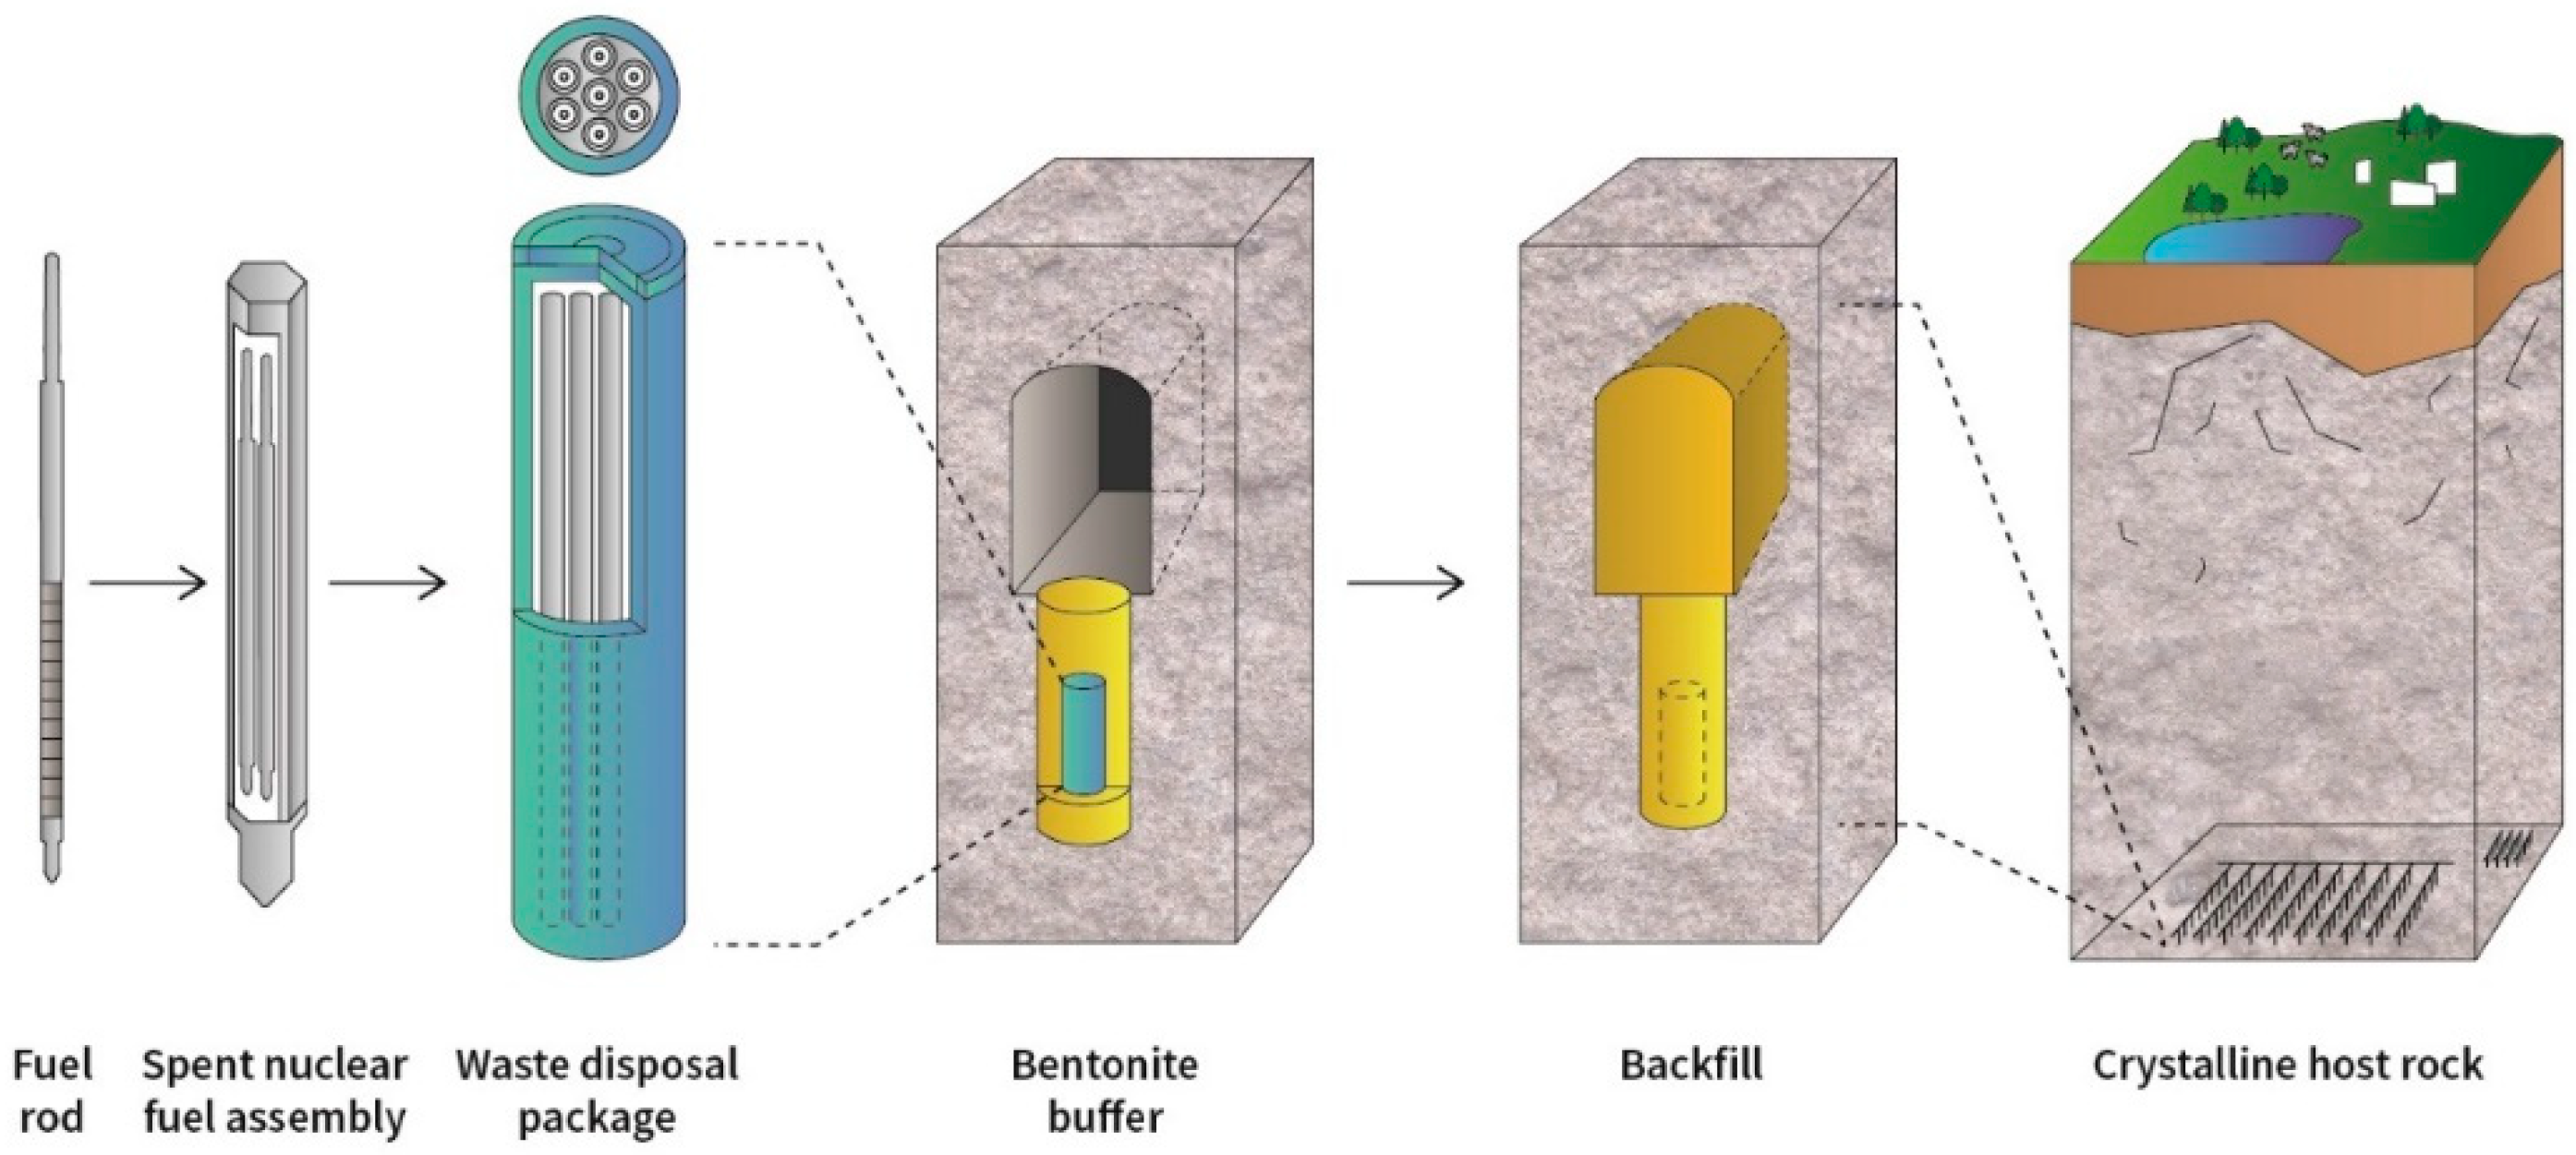
\includegraphics[width=0.8\textwidth]{graphics/img_ugn/image1.png}
  \caption{An example of vertical concept. Source file: \url{https://surao.gov.cz/presskit/ke-stazeni/}}
  \label{fig:image1}
\end{figure}

The storage sections will consist of access tunnels, in which \textit{vertical} waste disposal wells will be located. Only one \gls{WDP} is always located in each well. It is surrounded by a bentonite \textit{buffer} and a bentonite spacer block is placed between it and the well mouth. After the disposal wells are filled, the access tunnel is filled with \textit{backfill} and permanently closed with a sealing plug, see Figure \ref{fig:image1}.
The number of \gls{WDP}s, the axial distance between the access tunnels, and the number of tunnels will be determined in the future and will depend on the selected location.

The access tunnels are designed so that a transport service is possible during the \gls{WDP} loading. The tunnel must be free of significant disturbances and active water inflows (exact criteria will be specified in the future). After filling all the vertical boreholes, they will be filled with a backfill material specified below and finally closed with a sealing pressure plug. We assume that the access tunnel for the vertical disposal concept can be implemented conventionally, using the principles of \acrfull{nrtm}, see Figure \ref{fig:image6}. For more details, we refer to \cite{Hausmannova2023technical,Dohnalkova2022technicke}.

\begin{figure}[!htbp]
  \centering
  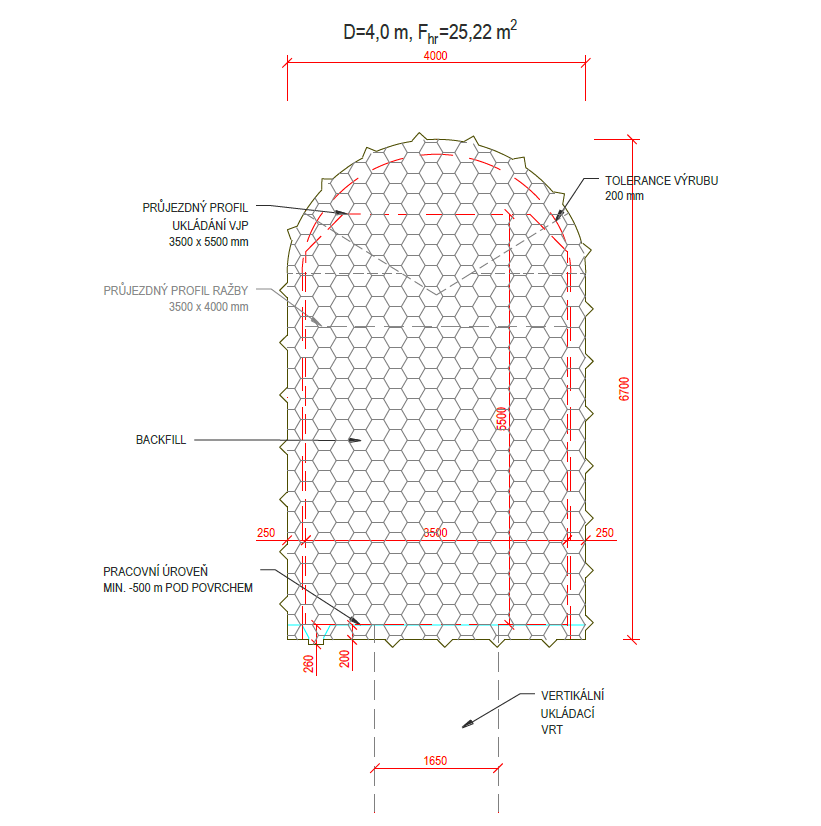
\includegraphics[width=0.8\textwidth]{graphics/img_ugn/image6.png}
  \caption{Backfilled access tunnel – subvariant 02 \acrshort{nrtm}.}
  \label{fig:image6}
\end{figure}


\subsection{Backfill and its expected properties}

The access tunnel will be filled mechanically. The filling machine will transport the pelletized material from the transport containers to the placement location using pneumatic (blowing) or mechanical transport (belt, screw conveyor). If necessary, the machine will perform working lining of the tunnel and/or vibratory compaction during execution. It is assumed that the access tunnel will be gradually filled from its previously closed end towards the future plug.

The backfill material must ensure that there is no excessive displacement of the material from the disposal well (sufficient support against swelling of the buffer). It must also ensure that the transport of water and radionuclides through the backfill is minimized. However, at the same time, it must allow gas to escape from the buffer without impairing the function of the backfill.

The backfill for the Czech deposition concept is made from the pelletized \acrshort{BCV} bentonite. To achieve the aforementioned requirements, the following backfill and pellet parameters have been suggested in \cite{Svoboda2023navrh}:

\noindent
\textbf{Backfill:}
\begin{itemize}
    \item Average dry density after placement to the access tunnels: $\rho_d=1400\,$kg/m$^3$;
    \item Moisture after placement: value not yet determined;
    \item Form: pellets.
\end{itemize}
\textbf{Pellets:}
\begin{itemize}
    \item Dry density: more than $2000\,$kg/m$^3$;
    \item Moisture: value not yet determined;
    \item Grain size: not yet determined.
\end{itemize}


\subsection{Pellet pressing technology}

It is a challenge to prepare manufacturally a sufficiently large amount of a pelletized \acrshort{BCV} bentonite backfill with the aforementioned properties. The current solution and ideas have been introduced in \cite{Stastka2020navrh}. We briefly summarize the main findings of this report.

% The production of pellets for deep nuclear waste repository, which is considered here, often refers in concepts to the production of homogeneous pressed stones from clay material (often bentonite). The produced pellets will be transported to the deep disposal site, where they will be used as part of the backfill system around the storage of radioactive waste packaging assemblies. They can be placed directly into the loading tunnels, which are used for the supply and installation of backfill layers \cite{Stastka2020navrh}.

% Industrially mined and processed (homogenized) bentonite will be used for the backfill. This will be supplied by the manufacturer in pelletized form with a suitable grain size composition. The material prepared in this way will be stored in suitable conditions until use. The pelletized material does not need to be modified before use and will be transported to the storage location in suitable transport containers.

% Pellets are made from selected clay material, which is first treated (e.g. dried and pre-homogenized) and then pressed under high pressure. The process is designed to produce solid, uniform and precisely shaped cylindrical pellets. An important parameter is the optimal moisture content of the material, which ensures good ability of bentonite to swell when in contact with water and subsequently create an uninterrupted barrier.

% Pellets simplifies the installation of bentonite-based component of the engineered barrier system that isolates radioactive waste. Pellets, typically less than 10 mm in size, can take various shapes—cylindrical, pillow-shaped, or irregular—and are produced through high-pressure compaction. This results in materials with very high density, strong swelling capacity, and low permeability.
% Pellet-based barriers can have varied compositions. They may consist solely of pellets, mixtures of pellets and powder, or compacted powder obtained by crushing pellets.

% In normal production operation, the compactor is used to process pelletized bentonite according to the requirements for the final product of production. This means that the material that is so-called oversized and undersized from the previous production phase is returned to the compactor. Both of these “production wastes” are crushed in a hammer crusher before being pressed in the compactor. Therefore, material with a grain size that cannot be used (is not used) as the final product of production is pressed in the compactor.

A key ingredient of the pellet pressing technology is the so-called \textit{compactor}, which was used for the pilot production of pellets. Its scheme is depicted in Fig. \ref{fig:image2}. Bentonite is fed to the rollers from above by a vertical screw conveyor. The compactor presses bentonite pellets in the form of plates with a thickness of up to about 2 cm and an edge of up to several cm (see Fig. \ref{fig:image8}). These plates are referred to as \textit{lenses} in production. 

\begin{figure}[!htbp]
  \centering
  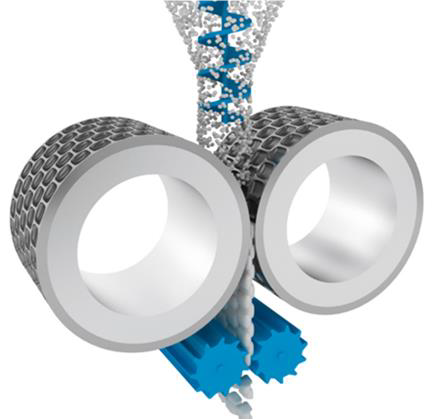
\includegraphics[width=0.7\textwidth]{graphics/img_ugn/image2.png}
  \caption{Scheme of press rollers with perforation located in the compactor.}
  \label{fig:image2}
\end{figure}
 
\begin{figure}[!htbp]
  \centering
  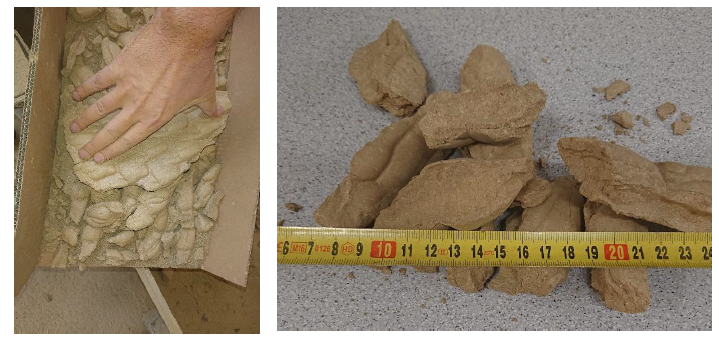
\includegraphics[width=0.8\textwidth]{graphics/img_ugn/image8.png}
  \caption{Photo of material pressed by a compactor, the so-called lens marked \acrfull{m181}; on the left during sample collection in the treatment plant and on the right in the \acrfull{ceg} laboratory.}
  \label{fig:image8}
\end{figure}

The next important ingredient is a \textit{hammer crusher} that crushes the lenses. The crushed material can then be sieved into the required grain-size fractions. The specific dimensions are chosen with regard to the required swelling capacity and effective use of space. Pellets with inconvenient grain sizes require repeated pressing. The resulting pelletized materials, marked \acrfull{m182-0-8} and \acrfull{m182-0-50}, are depicted Fig. \ref{fig:image10} and Fig. \ref{fig:image9}. Their grain sizes are 0-8 mm and 0-50 mm, respectively.

\begin{figure}[!htbp]
  \centering
  \begin{minipage}{0.48\textwidth}
    \centering
    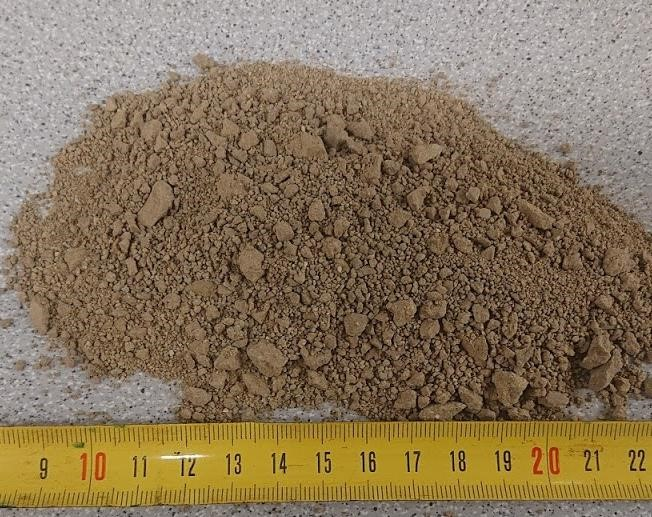
\includegraphics[width=\textwidth]{graphics/img_ugn/image10.jpg}
    \caption{Pelletized bentonite marked \acrshort{m182-0-8}.}
    \label{fig:image10}
  \end{minipage}  
  \hfill
  \begin{minipage}{0.48\textwidth}
    \centering
    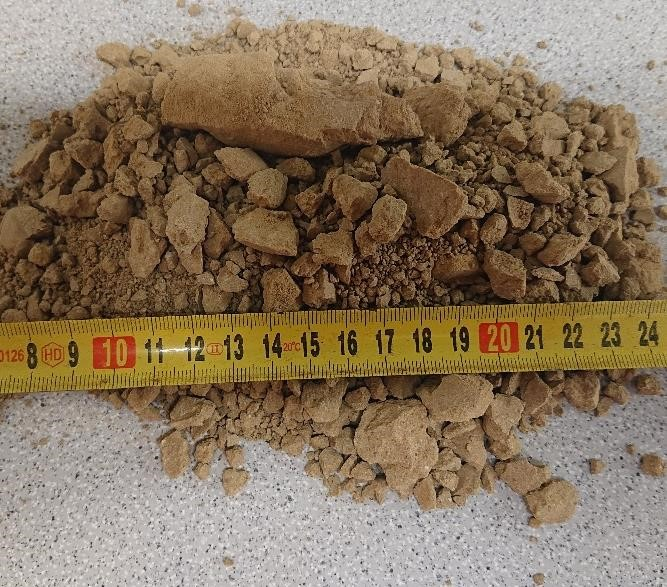
\includegraphics[width=\textwidth]{graphics/img_ugn/image9.jpg}
    \caption{Pelletized bentonite marked \acrshort{m182-0-50}.}
    \label{fig:image9}
  \end{minipage}
\end{figure}

\acrshort{m182-0-8} and \acrshort{m182-0-50} materials were further analyzed. After a few modifications of the technology, it was found that the pellet dry density is above $2000\,$kg/m$^3$ as required. Their moisture contents are about $4-5~\%$. 

\renewcommand{\arraystretch}{1.2} % optional: makes rows a bit taller for readability

\begin{table}[!htbp]
\centering
\caption{Compaction results for pelletized bentonite from the seventh industrial production batch.}
\label{tab:compaction}
\begin{tabularx}{\textwidth}{|>{\centering\arraybackslash}l|>{\centering\arraybackslash}c|>{\centering\arraybackslash}c|>{\centering\arraybackslash}c|>{\centering\arraybackslash}X|}
\hline
\textbf{Material} & \multicolumn{3}{c|}{\textbf{Dry Density} \(\rho_d\) [\(\mathrm{g/cm^3}\)]} & \textbf{Compaction Method (Cylinder Volume)} \\ \hline
\multicolumn{5}{|c|}{\textbf{Pelletized bentonite, \(w=4.6~\%\), \(\rho_{d,\mathrm{pellets}}=2.01\,\mathrm{g/cm^3}\)}} \\ \hline
\textbf{\acrshort{m182-0-50}} & 1.40 & 1.42 & 1.41 & Free poured (120\,dm\(^3\)) \\ \cline{2-5}
                        & 1.48 & 1.50 & 1.50 & Shaken (120\,dm\(^3\)) \\ \cline{2-5}
                        & 1.62 &      &      & Compacted with piston (60\,kg) in \(\sim10\,\mathrm{cm}\) layers (120\,dm\(^3\)) \\ \cline{2-5}
                        &      & 1.65 & 1.64 & Compacted with piston (60\,kg) in \(5\,\mathrm{cm}\) layers (120\,dm\(^3\)) \\ \hline
\textbf{\acrshort{m182-0-8}}  & 1.26 & 1.23 & 1.22 & Free poured (120\,dm\(^3\)) \\ \cline{2-5}
                        & 1.36 & 1.32 & 1.33 & Shaken (120\,dm\(^3\)) \\ \cline{2-5}
                        & 1.51 &      &      & Compacted with piston (60\,kg) in \(\sim10\,\mathrm{cm}\) layers (120\,dm\(^3\)) \\ \cline{2-5}
                        &      & 1.55 & 1.55 & Compacted with piston (60\,kg) in \(5\,\mathrm{cm}\) layers (120\,dm\(^3\)) \\ \hline
\end{tabularx}
\end{table}

Next laboratory experiments were focused on the determination of average dry density of the pelletized bentonites \acrshort{m182-0-8} and \acrshort{m182-0-50} subjected to compaction, which is planned in the access tunnels. Compaction tests were conducted under \textquote{semi-operational} conditions, as tens of kilograms of pelletized bentonite were compacted in a steel cylinder with a volume of~\(120\,\mathrm{dm^3}\). During compaction, various methods were tested, namely free pouring, \textquote{shaking} by manual movements of the cylinder, and compaction of pellets by falling with a steel rammer. The results are summarized in Tab.~\ref{tab:compaction}.

We see that the required average dry density \(1.4\,\mathrm{g/cm^3}\) is achieved for \acrshort{m182-0-50} and any compaction method. In case of \acrshort{m182-0-8}, the required density is achieved only for the compaction with a steel rammer.

It is important to note that the compaction under laboratory conditions is not representative for backfilling emplacement drifts, where the material will be placed 
horizontally along irregular tunnel walls, transported over several tens of meters, and 
subjected to large-scale self-compaction, arching, segregation of grain-size fractions, 
and potential void formation. A full-scale or large-box experiment with horizontal emplacement should be used to characterize the backfill density distribution and compaction behavior under realistic geometric and operational constraints.

\subsection{Evaluation of hydraulic conductivity and swelling pressure} 

The next aim was to analyze the dependence of hydraulic conductivity and swelling pressure on the average dry density of M182. For this study, only the M182 0-8 mm material was used, see \cite{Stastka2020navrh} . The evaluation was conducted in accordance with the supplier's internal methodologies, based on valid technical standards. However, the swelling pressure tests were not completed in a standard manner, and therefore it was necessary to determine the swelling pressure by reducing the total stress from the conclusion of the test (by approximately $3-15~\%$).

The~dependence of hydraulic conductivity on the average dry density is depicted in Fig.~\ref{fig:image_hyd_vod}. The trend indicates that increasing dry density leads to decreasing hydraulic conductivity.
\begin{figure}[!htbp]
  \centering
  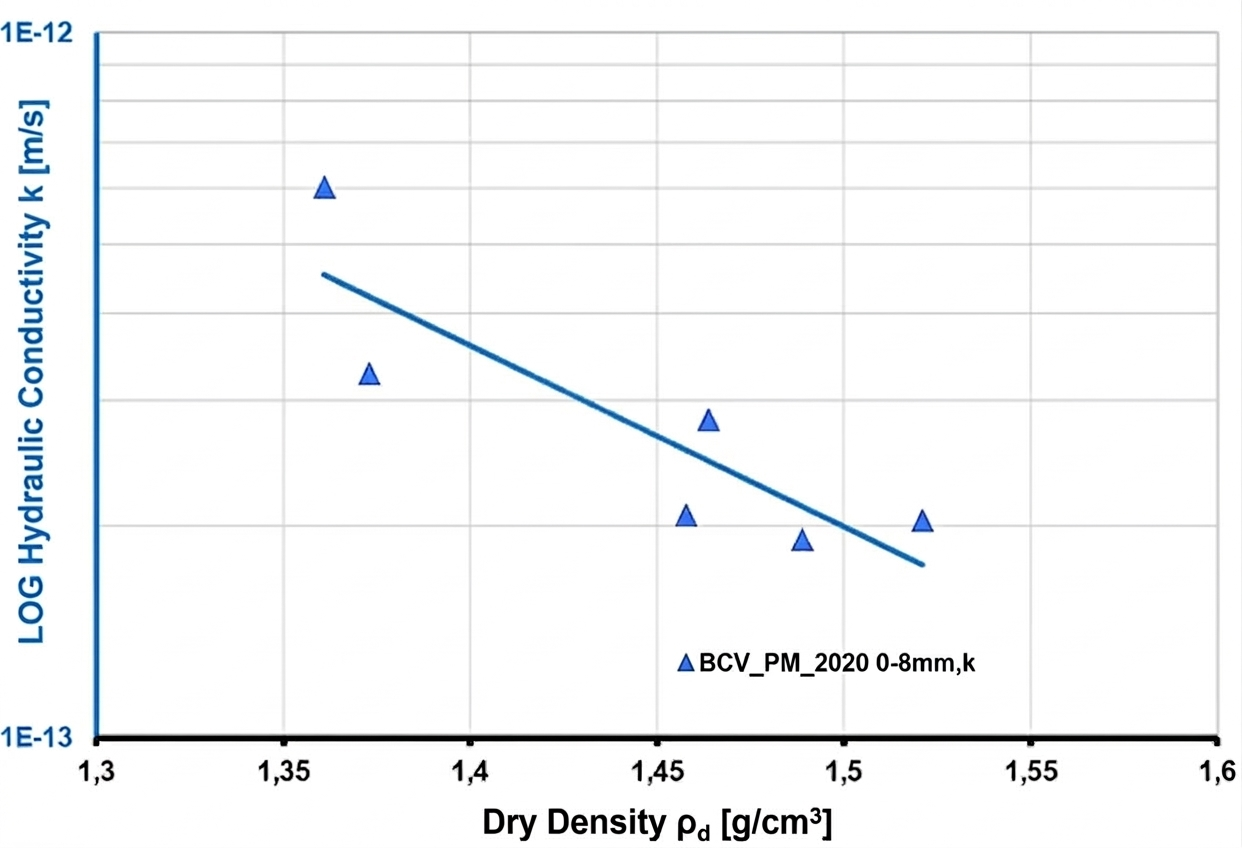
\includegraphics[width=0.8\textwidth]{graphics/img_ugn/Cimage_hyd_vod.png}
  \caption{Dependence of hydraulic conductivity $k$ (logarithmic scale) on dry density \(\rho_d\) for bentonite material \texttt{\acrshort{m182-0-8}}.}
  \label{fig:image_hyd_vod}
\end{figure}

The graph in Figure~\ref{fig:image14} illustrates the relationship between the dry density \(\rho_d\) and the swelling pressure \(\sigma_\text{sw}\) of M182 0-8 mm. As the dry density increases from approximately 1.3~g/cm\(^3\) to 1.5~g/cm\(^3\), a significant rise in the swelling pressure is observed, with maximum values exceeding 6~MPa. The fitted curve suggests an exponential dependency, highlighting that even minor increases in dry density result in considerable improvements in swelling pressure.

\begin{figure}[!htbp]
  \centering
  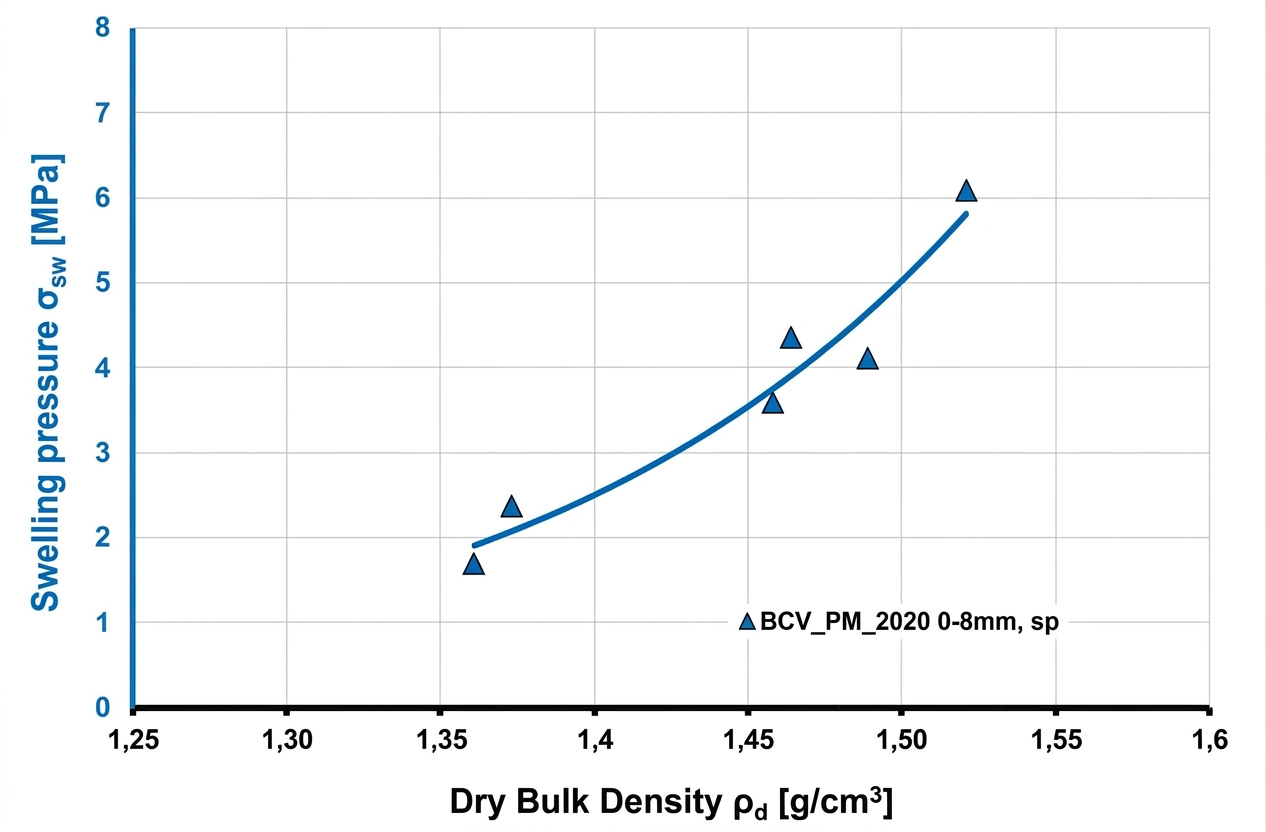
\includegraphics[width=0.8\textwidth]{graphics/img_ugn/Cimage14.png}
  \caption{Dependence of swelling pressure \(\sigma_\text{sw}\) on dry density \(\rho_d\) for pelletized bentonite material \texttt{\acrshort{m182-0-8}}. The swelling pressure increases significantly with higher dry density.}
  \label{fig:image14}
\end{figure}

This behavior confirms that the developed pelletized bentonite material exhibits the required properties for use as a buffer and sealing component in the construction of deep geological repositories for radioactive waste. The combination of high swelling pressure and appropriate grain size distribution ensures effective mechanical stability and minimizes potential pathways for radionuclide migration.

Furthermore, Figure~\ref{fig:image15} presents a comparative analysis of the hydro-mechanical behavior of pelletized and initial non-pelletized bentonite. These two materials are denoted as \texttt{M182 0-8 BCV\_PM\_2020} and \texttt{BCV\_PM\_2017} within this study. For \texttt{BCV\_PM\_2017}, data from \cite{Cervinka2018kompletni,Svoboda2019interakcni} were used. The left vertical axis shows the hydraulic conductivity plotted on a logarithmic scale, while the right vertical axis corresponds to the swelling pressure.

\begin{figure}[!htbp]
  \centering
  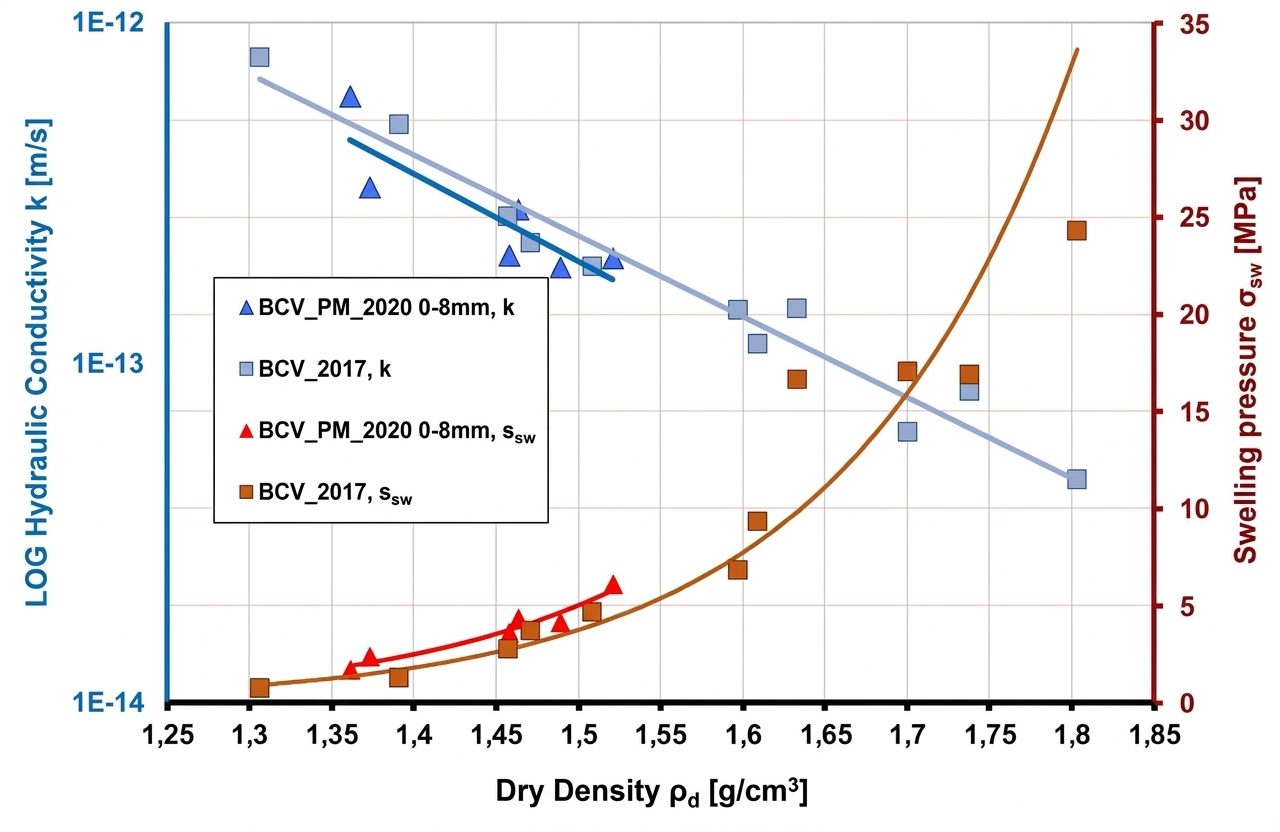
\includegraphics[width=0.8\textwidth]{graphics/img_ugn/Cimage15.png}
\caption{Comparison of the relationship between dry density \(\rho_d\) and hydraulic conductivity $k$ (left axis) and swelling pressure (right axis) for pelletized bentonite materials BCV\_PM\_2020. Results are compared to non-pelletized ground bentonite BCV\_2017.}
  \label{fig:image15}
\end{figure}
 
The results (dependencies) for both compared materials appear to be similar. For both materials, a clear trend is observed in which an increase in dry density \(\rho_d\) results in a significant reduction in hydraulic conductivity and a simultaneous exponential increase in swelling pressure. The \texttt{M182 0-8 BCV\_PM\_2020} material exhibits slightly lower hydraulic conductivity and relatively moderate swelling pressures compared to the \texttt{BCV\_PM\_2017} material across the range of densities tested. This indicates that the pelletized bentonite (\texttt{BCV\_PM\_2020}) has favorable properties for use as a backfill material in deep geological repositories for radioactive waste, combining low permeability with adequate swelling capacity.

Finally, it is important to highlight that all hydraulic conductivity and swelling-pressure tests reported in Figs.~\ref{fig:image_hyd_vod}–\ref{fig:image15} were performed under fully saturated conditions (constant-volume saturation). Therefore, the reported values of 
$\sigma_{\text{sw}}$ correspond to the equilibrium swelling pressure in the 
saturated state.


\subsection{Concluding remarks to achieved hydro-mechanical properties of the BCV pelletized backfill}

Currently, we have the following requirements on the \acrshort{BCV} pelletized backfill for the Czech deposition concept: 
\begin{enumerate}
    \item Dry density of pellets should be greater than $2000 \munit{kg/m^3}$;
    \item Average dry density of the backfill after placement to the access tunnels\\ should be $1400 \munit{kg/m^3}$.
\end{enumerate}
The suggested pellet pressing technology enables us to prepare the pelletized \texttt{M182 0-8 mm} and \texttt{M182 0-50 mm} materials satisfying the first requirement. The average dry density of these materials has been analyzed only via laboratory compaction tests, which is not able to catch the complexity of in situ conditions. From the performed laboratory experiments, it follows that the required average density of $1400\,$kg/m$^3$ is achieved for \texttt{M182 0-50 mm} using all compaction methods. However, for \texttt{M182 0-8 mm}, only some compaction methods give this required value.

Next, the hydraulic conductivity and swelling pressure of the pelletized BSV bentonite have been analyzed under laboratory conditions and for the \texttt{M182 0-8 mm} material. 
From these measurements, the hydraulic conductivity and swelling pressure for fully saturated pellets at an average dry density of 
$\rho_d = 1400 \ \mathrm{kg/m^3}$
can be roughly estimated as:
$k = (3.5\text{–}5) \times 10^{-13} \ \mathrm{m/s}, \quad p_s = 1.5\text{–}2.5 \ \mathrm{MPa}$.
For \texttt{M182 0-50 mm}, no measurements of the hydro-mechanical (HM) parameters of the pellets have been performed. Such measurements could be helpful from the perspective of possible preferential flow paths (zones with higher hydraulic conductivity) in the backfill. 

The aforementioned analyses are not representative of backfilling emplacement drifts, where the material will be placed horizontally along irregular tunnel walls, transported over several tens of meters, and subjected to large-scale self-compaction, arching, segregation of grain-size fractions, and potential void formation. A full-scale or large box experiment with horizontal emplacement should be used to characterize backfill density distribution, compaction behavior, and hydro-mechanical properties under realistic geometrical and operational constraints.

More comprehensive analyses can be found in several international studies. In the next section, we summarize selected experiences with FEBEX and MX-80 bentonites and related pelletized material. Their knowledge may complete missing properties of the backfill and may be inspirational for future analyses of the \acrshort{BCV} pelletized material.


%----------------------------------

\section{Macro-scale properties of bentonite backfill}
\label{sec_advanced}

\subsection{Distribution of bentonite pellets in access tunnels}


% \sts{[Standa: V prvnni casti teto podsekce chybi citace! Navic mi pride, ze tato cast je pro nase ukoly bezpredmetna, dokud nebude proveden relavantni in situ experiment. Doporucil bych prvni cast teto sekce uplne vynechat.]}

The distribution of bentonite pellets in the filling of access tunnels of a deep radioactive waste repository is a key parameter affecting the resulting dry density (\textit{dry density}), and thus the functionality of engineering barriers. A properly designed distribution system should ensure a high degree of homogeneity of the resulting filling layer, minimizing gaps and effective long-term function of the entire repository.

Pellet material is typically deposited in access tunnels in a modular manner, for example in layers or blocks. The aim is to minimize the formation of large voids and ensure uniform coverage of the area in contact with the surrounding rock. Optimal distribution not only supports effective heat removal from \gls{WDP}, but also reduces the likelihood of hydrological anomalies that could negatively affect the migration paths for radionuclides.

The distribution process can be carried out mechanically, for example using screw conveyors. The method of placement significantly influences the resulting distribution of dry density, as the mechanics of materials are subject to specific laws (for example, the angle of repose or the transfer of pressures between particles).

\textbf{Mechanics of materials and local variability}

\begin{itemize}
\item \textbf{Angle of repose and stability} \\
Each material (including bentonite pellets) has its own characteristic angle of repose, at which the particles spontaneously settle. During free pouring, areas with lower and higher density are created depending on local conditions, especially the geometry of the passage and the properties of the particles, \cite{SKB:TR-12-06}.
\item \textbf{Janssen effect} \\
In vertical or inclined spaces (for example, when filling chambers slowly), part of the vertical load is taken by the walls due to the transfer of forces between the particles and the peripheral envelope. The resulting stress and therefore the local compaction differ at different points of the perpendicular cross-section, \cite{Janssen:1895}.
\item \textbf{Arching and percolation} \\
Local supports and ‘arches’ created during pouring can cause some areas to remain less compacted, while others become significantly more compacted. This effect causes increased variability in the distribution of pellets and dry density within a single corridor or layer, \cite{Terzaghi:1943}.
\end{itemize}

\textbf{Dynamics of initial and final dry density}

After the initial filling of access tunnels by free pouring, it is natural to expect the formation of horizontal and vertical gradients of dry density. The mechanical nature of the movement and settlement of pellets, their different sizes and shapes, and friction itself cause the density to be lower in some areas (especially in the lower parts and near the contact surfaces), while it may be higher in the upper/V-planes.

With the formation of a network of contacts between pellets, self-compression also occurs - some areas become more compacted by their own weight. After the filling is completed, further leveling of the distribution occurs gradually, especially with the onset of bentonite hydration.

\subsection{Expected stress on tunnel walls induced by backfill}

Fully saturated \acrshort{BCV} pellet backfill at an average dry density 
$\rho_d = 1400~\mathrm{kg/m^3}$ develops a laboratory swelling pressure in the range
$\sigma_{\text{sw}} \approx 1.5\text{–}2.5~\mathrm{MPa}$ under rigid constant-volume 
boundary conditions. These values are inferred from the measured hydraulic conductivity 
and swelling-pressure data for the 0--8~mm fraction (Figs.~\ref{fig:image_hyd_vod} and 
\ref{fig:image14}) and correspond to full saturation.

In a real emplacement drift, part of the swelling capacity is consumed by
\begin{enumerate}
    \item closure of initial voids near the tunnel ceiling, 
    \item compaction of the pellet layer itself, and  
    \item deformation of the \Gls{EDZ} and \Gls{EIZ}surrounding the tunnel (see \ref{sec:hm_steady}.
\end{enumerate}


Based on comparisons with KBS-3 tunnel backfill concepts, where long-term radial pressures 
of $0.2\text{–}1.0$~\unit\MPa~ are considered sufficient for rock support and sealing, see \cite{SKB:2010:TR-10-12}
A realistic and conservative estimate for the Czech concept is at the lower bound, $\sigma_{\text{sw}} \approx \SI{1.5}{\MPa}$, due to the above-mentioned reasons.

% This design value should be used in the coupled HM and \Gls{EDZ} transport simulations in 
% Subsequent Chapters 4-7 [LINK], where mechanical interaction between the backfill and the 
% \Gls{EDZ} will be resolved explicitly. Simply the pressure on the wall $p_r = \sigma_{\text{sw}} + h \rho_{w} g$, where $h$ is the depth of backfill, $\rho_{w}$ is the density of the water, and $g$ is the acceleration due to gravity. But for the experiment the hydrostatic pressure (the pressure exerted by a fluid at rest due to gravity) is neglected, since URF Bukov is not under water.

% \sts{[Standa: Je vztah $p_r = \sigma_{\text{sw}} + h \rho_{w} g$ podlozeny literaturou? Moc se mi to nepozdava, protoze zde chybi v bilanci jeste napetovy stav zpousobeny razbou. URF Bukov je zde trochu vytrzeny z kontextu.]}

\subsection{Hydration and long-term pore distribution}
\label{sec:pore_distr}
Bentonite reacts to the presence of water by significant swelling, which gradually leads to filling of gaps, overcoming of initial density gradients and, thanks to expansion forces, to equalizing of internal stress in the entire layer. The result of long-term hydration is the creation of an almost homogeneous, tight barrier with a minimum of voids.

Pelletized bentonite samples exhibit a complex, multi-modal porous structure, as demonstrated by several studies~(\cite{Hoffmann2007hydro}). This structure has been characterized using techniques such as Mercury Intrusion Porosimetry (MIP) and X-ray computed microtomography. At the scale of an individual pellet, a distinct double porosity system is observed~(\cite{Hoffmann2007hydro}). This dual structure arises from the compaction process applied on the dry side of the optimum moisture content during pellet production.

Figure~\ref{fig:hoffman}~(b) illustrates the bimodal pore size distribution (PSD) of a highly compacted pellet with a dry density $\rho_d = 1.95~\mathrm{Mg/m^3}$. Two dominant pore families are identified: intra-aggregate pores (approximately $13~\mathrm{nm}$) and inter-aggregate pores (approximately $3~\mu\mathrm{m}$). A~similar bimodal PSD was reported by~\cite{MolineroGuerra2017} for an MX-80 bentonite pellet compacted to $\rho_d = 2.06~\mathrm{Mg/m^3}$ and subjected to a suction of $135~\mathrm{MPa}$. Notably, the inter-aggregate pores in this case, with an average diameter of approximately $4$–$5~\mu\mathrm{m}$, accounted for only about $7~\%$ of the total porosity.
\begin{figure}[!htbp]
  \centering
  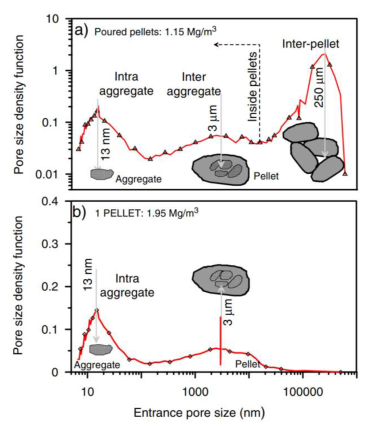
\includegraphics[width=0.7\textwidth]{graphics/img_ugn/hoffman.png}
\caption{PSD of FEBEX bentonite in: a) a compacted sample, and b) a single pellet (\cite{guilia}).}
  \label{fig:hoffman}
\end{figure}

Larger-scale pellet assemblies present even more complex porosity patterns. Figure~\ref{fig:hoffman}~(a) shows the PSD of a sample composed of multiple pellets compacted using a gravity fall method ($\rho_d = 1.15~\mathrm{Mg/m^3}$). This sample displays a trimodal PSD with characteristic pore sizes at approximately $13~\mathrm{nm}$, $3~\mu\mathrm{m}$, and $250~\mu\mathrm{m}$. The largest mode corresponds to inter-pellet voids. Additional larger voids may also exist due to irregular pellet packing; however, these are beyond the detection range of MIP, which is limited to pore entrance diameters up to $500~\mu\mathrm{m}$~(\cite{Hoffmann2007hydro}).

Moreover, the maximum void ratio measured by MIP tends to underestimate the actual total void ratio. This discrepancy is attributed to the presence of so-called \textit{infra-porosity}~(\cite{delage2008experimental}) --- extremely small pores with entrance diameters less than $5.4~\mathrm{nm}$, which are prevalent in heavily compacted pellets but inaccessible to mercury intrusion.






\subsection{Water retention behavior of pelletized FEBEX bentonite}

% \sts{[Standa: Je treba zduraznit, ze FEBEX (Spanelsko), MX-80 (USA) a GMZ (Cina) jsou ruzne typy bentonitu z ruznych zemi. Neprijde mi napr. korektni psat FEBEX (MX-80 type).]}
% JB: Mohlo by to být přesnější, ale FEBEX/MX-80 type se užívá i jinde, asi jde tedy o podobný typ bentonitu. 

We have not found in the literature the water retention curve for pelletized BVC bentonite, hence only pelletized FEBEX Bentonite (Spain) \cite{Mayor2005} or GMZ (China) \cite{Liu2021} is mentioned.
In experiments on FEBEX using MX-80 type bentonite (USA) in pellet/powder form, water retention curves (WRC) have been measured and modeled. For example, \cite{Mayor2005} reported WRCs for a pellet mixture ($4 \munit{mm}$ FEBEX pellets) at dry densities of $1.30$, $1.50$, and $1.90 \munit{Mg/m^3}$. These curves (fitted with a van Genuchten model) show that higher-density pellet fills retain more water at a given suction. He et al. (2020) measured WRCs for the MX-80 pellet skeleton (estimated from MIP data) and for crushed MX-80 powder under wetting. They found the pellet WRC has a much higher air-entry value than the blocks: an entry suction $P_0 \approx 35 \munit{MPa}$ for the pellet structure vs. $\approx 2 \munit{MPa}$ for the powder (\cite{mesa2020microstructural}). A mixed bentonite with $80~\%$ pellets/$20~\%$ powder (dry density $\sim 1.49 \munit{Mg/m^3}$) had an intermediate $P_0 \approx 10 \munit{MPa}$ (\cite{mesa2020microstructural}). Notably, at very low water contents ($<10~\%$), the retention curves for pellet and powder converge (becoming insensitive to void ratio), see \cite{mesa2020microstructural}. In other words, above $\sim 10 \munit{MPa}$ suction (dry states) both pellet and fine powders hold similar adsorbed water, but at lower suction (higher water content) the pellets’ large pores cause the pellet mixture to store less water than dense blocks.


Recent studies comparing pelletized and compacted bentonite confirm this trend. \cite{Liu2021} compared the WRCs of GMZ bentonite in three forms: a mixture of constant-volumes of pellets, a compacted block (the same density $\sim 1.45 \munit{Mg/m^3}$), and a free-swelling pellet. They found all three behave similarly at high suctions ($>10 \munit{MPa}$), but pellet mixtures retain less water at low suction ($<10 \munit{MPa}$) than a dense block of the same clay (\cite{Liu}). Physically, this is because at low suctions the compacted block stores extra capillary water in its finer pores, whereas the pellet fill’s water is largely confined to the clay particle micropores and the (initially dry) larger inter-pellet channels. Correspondingly, the pellet mixture exhibited a lower overall water content during early hydration. These results emphasize that initially heterogeneous pellet fabric yields a distinctive WRC: the pellet mixture and compacted block curves converge at high suction (where adsorptive water dominates), but diverge when capillary water enters (low suctions), see \cite{Liu}. In particular, in post-mortem tests of the heated barrier in situ of FEBEX, bentonite blocks exposed to up to $\sim 150 \munit{{}^\circ C}$ did not show any permanent change in the WRC: the water retention capacity of the blocks remained basically the same as before the test (\cite{villar2021febex}).


In the early stage after emplacement, the pellet backfill is unsaturated, and the hydraulic processes are complex. Inflowing groundwater tends to be captured in the macro-voids of the pellet pack before fully entering clay micropores. For example, field- and lab-scale studies show that a large fraction of incident water can be temporarily stored in inter-pellet gaps (on the order of tens of percent of pore volume), see \cite{SKB2009}. SKB/Posiva analyses for KBS-3 tunnels highlight that inflow rates up to $\sim 0.5 \munit{l/min}$ can be safely absorbed in the pellet gap between blocks and rock (\cite{SKB2009}). During this phase, the pellet fill evolves (pellets swell, powder moves slightly, macrovoids shrink), gradually raising the suction in the remaining pores. Only once macropores fill and saturation nears will the retention curve shift to the final high-water branch. Because of the initially high void ratio and low matric suction, gas phase and air displacement can also be significant early on. Overall, studies agree that pelletized fills absorb water more quickly through the large pores, but saturate more heterogeneously, compared to massive blocks (\cite{SKB2009}). This is reflected in the water retention curve in Fig.~\ref{fig:image24}. Note that from Fig.~\ref{fig:image24} we can compute the volume of water over-saturation volume (against water density = $1 \munit{Mg/m^3}$) is injected above the expected water pore space. For dry density $1.9 \munit{Mg/m^3}$ is to by experience around $60~\%$ more,  dry density 
$1.7 \munit{Mg/m^3}$ is to by experience $28~\%$, and $\rho_d = 1.7 \munit{Mg/m^3}$ has around $20~\%$  of water more.

\begin{figure}[!htbp]
  \centering
  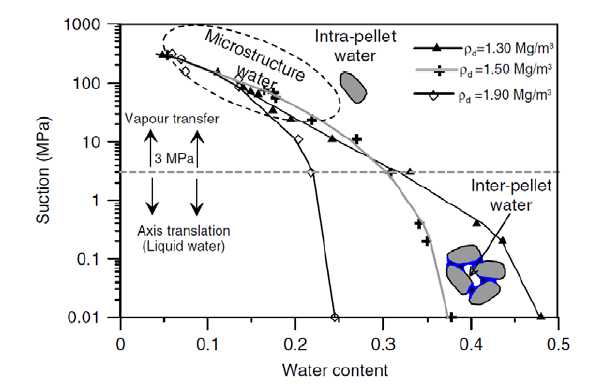
\includegraphics[width=0.8\textwidth]{graphics/img_ugn/image24.png}
\caption{Water retention curves upon wetting of pellet samples compacted to different dry density values of $1.3$, $1.5$, and $1.9 \munit{Mg/m^3}$, \cite{Hoffmann2007hydro}. Compare with Fig.~\ref{fig:hoffman} to see the distribution of porosity.}
  \label{fig:image24}
\end{figure}


% \sts{[Standa: Zrnitostni krivky pro ruzne typy M182 (peletizovany BCV bentonit) jsou take uvedeny ve \cite{Stastka2020navrh}. Neni mi ale znama souvislost s porozitou a difúzní a disperzní parametry.]}
% JB: Zrinitosntí krivky jsou pro suchou smes, po hydrataci bude stav uplně jiný.


\subsection{Advanced hydraulic properties}

It was originally assumed that the permeability of pellets is higher than the permeability of blocks at the same \(\rho_d\) - this was not confirmed by in situ EB measurements, see \cite{osti_1762807}. Fig.~\ref{fig:image16} illustrates the dependence of hydraulic permeability \(k_\text{w}\) on the dry density \(\rho_d\) for two types of materials: pelletized bentonite and compacted FEBEX bentonite.

As expected, the permeability of both materials decreases significantly with increasing dry density. The pelletized bentonite shows a slightly higher permeability at comparable densities when compared to the compacted FEBEX bentonite, which is consistent with the expected behavior due to the initial porosity and microstructural differences.

The results demonstrate that sufficiently compacted pelletized bentonite can reach permeability values close to those of FEBEX bentonite, a reference material for engineered barrier systems in nuclear waste repositories. These findings support the use of pelletized bentonite for backfilling and sealing, provided that adequate dry density is achieved during emplacement.

The clear trend observed in the graph also reinforces the importance of dry density as a key design parameter for achieving the required hydraulic performance in bentonite-based barrier systems.
\begin{figure}[!htbp]
  \centering
  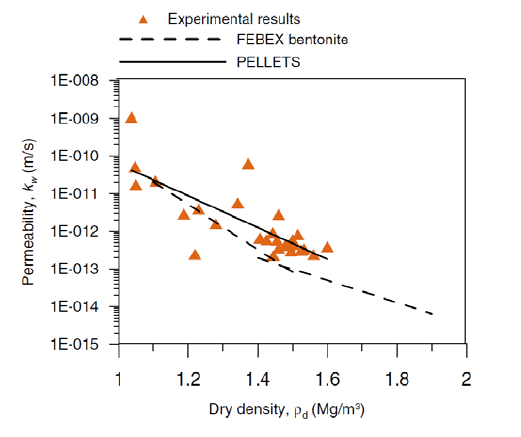
\includegraphics[width=0.8\textwidth]{graphics/img_ugn/image16.png}
\caption{Dependence of permeability $k_w \,\bunit{m/s}$ on dry density $\rho_d \,\bunit{Mg/m^3}$ for pelletized bentonite material and compacted FEBEX bentonite (based on laboratory tests only).}
  \label{fig:image16}
\end{figure}
The hydraulic conductivities measured in the \acrfull{GBM} samples ranged from 
\(8 \times 10^{-12}\) to \(2 \times 10^{-13}\,\mathrm{m/s}\) in Fig.~\ref{fig:image16}. These values were determined using Pearson water as the permeating fluid, see Fig.~\ref{fig:image17}. 
\begin{figure}[!htbp]
  \centering
  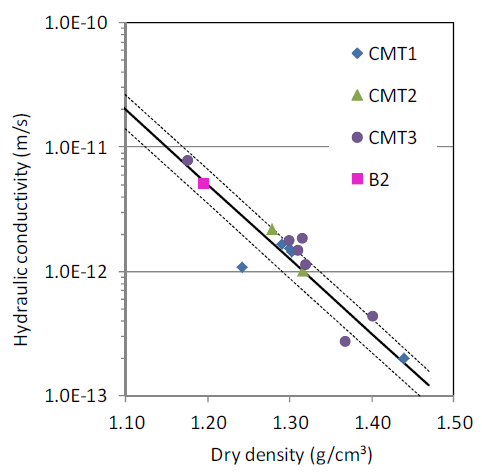
\includegraphics[width=0.6\textwidth]{graphics/img_ugn/image17.png}
\caption{Hydraulic conductivity determined with Pearson water in samples retrieved upon dismantling of the EB test (B-S samples) and empirical correlation for untreated FEBEX bentonite, \cite{villar2009thm}.}
  \label{fig:image17}
\end{figure}

Under full saturation, it can be assumed that homogenization of the pellets will occur, the upper void will close, and no zone with higher permeability will form. The main reason for this assumption comes from experimental observations where pellets with initially low saturation (gravimetric water content \(w = 4\text{–}5~\%\)) have very high permeability until the degree of saturation of bentonite pellets reaches \(S_r = 60\text{–}70~\%\) (see Fig.~\ref{fig:image25}, (\cite{Hoffmann2007hydro})). Water from the surrounding rock will initially infiltrate into the lower part of the drift. Pellets at the bottom will start swelling first, which will close the void in the upper part.

\begin{figure}[!htbp]
  \centering
  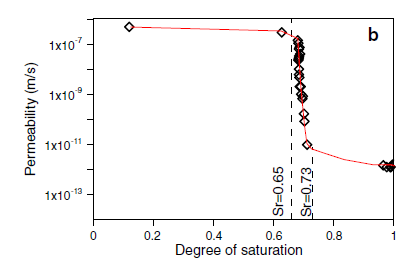
\includegraphics[width=0.6\textwidth]{graphics/img_ugn/image25.png}
\caption{Hydraulic conductivity of unsaturated bentonite MX-80 pellets, \cite{Hoffmann2007hydro}.}
  \label{fig:image25}
\end{figure}


A similar situation (\cite{BernachyBarbe2022beacon}, p.~112) was modelled within the EBS Task 13 Stage 2 project (see Appendix~1, Fig.~11), where the void above a FEBEX bentonite cylinder closed during water saturation from the bottom. The measured permeability at full saturation was even lower in the upper (previously void) section than in the lower section.







% \subsection{Transport Parameters of Saturated Pelletized Backfill}

% Near-field radionuclide transport in a saturated pelletized bentonite backfill is expected to be
% diffusion-dominated; any advection is restricted to early-time preferential pathways associated
% with the initial macro-void network and diminishes as swelling and resaturation homogenise the
% pore structure. The parameter set below is therefore structured around (i) porosity and pore-size
% statistics, (ii) diffusion-accessible porosity and tortuosity (linking $D_w$ to $D_e$), and
% (iii) a conservative treatment of hydrodynamic dispersion.

% \paragraph{Dry density as the primary state variable.}
% Large-scale emplacement tests demonstrate that the achievable installed dry density depends on
% pellet grading and mixture composition \cite{DixonEtAl2011_P1144}. In the absence of direct
% measurements for the exact $0$--$50$~mm fraction after in situ resaturation, we parameterise the
% transport properties as functions of the (measured) dry density $\rho_d$.

% \paragraph{Total porosity.}
% Using the measured solid density $\rho_s$ of the BCV bentonite (laboratory value),
% the total porosity is computed as
% \[
% n = 1 - \frac{\rho_d}{\rho_s}.
% \]
% For example, with $\rho_d = 1.4~\mathrm{Mg/m^3}$ and $\rho_s = 2.87~\mathrm{Mg/m^3}$,
% one obtains $n \approx 0.51$.

% \paragraph{Multi-modal pore structure and characteristic length scales.}
% Pellet mixtures exhibit a multi-modal pore system, with a clear separation between large
% (inter-pellet / gap-related) and small (intra-pellet / intra-aggregate) pore families
% \cite{NavarroEtAl2020_EngGeo105714,GramegnaEtAl2022_EngGeo106700}.
% In particular, MIP/post-mortem analyses show that very large pores present initially may
% disappear and transform into pore families with characteristic diameters of order
% $\sim 50~\mu\mathrm{m}$ and $\sim 200~\mathrm{nm}$ at the end of hydration tests
% \cite{GramegnaEtAl2022_EngGeo106700}.
% Complementary laboratory evidence on pellet/block systems highlights that macropores larger
% than $\sim 550~\mu\mathrm{m}$ can be relevant at early stages of saturation and transfer
% \cite{VillarEtAl2021_EngGeo106272}.
% For dispersion-related upscaling, these observations motivate two characteristic length scales:
% (i) a pore-network scale $\ell_p \sim 10^{-4}$--$10^{-3}$~m (order of macropore diameters),
% and (ii) a structural heterogeneity scale $\ell_s$ of order the pellet size (mm--cm), e.g.
% 7--32~mm in representative pellet-mixture tests \cite{GramegnaEtAl2022_EngGeo106700}.

% \paragraph{Diffusion-accessible porosity.}
% For neutral tracers and (most) cations, the diffusion-accessible porosity can be taken close to
% the total porosity, $\varepsilon \approx n$ \cite{VanLoon2014_NTB1203}.
% For anions, only a fraction of the pore space is accessible due to anion exclusion (notably from
% interlayer water), and $\varepsilon_{\mathrm{an}} < n$ \cite{VanLoon2014_NTB1203}.
% For safety-assessment style modelling, it is convenient to treat $\varepsilon_{\mathrm{an}}$
% as a calibrated (or bounded) fraction of $n$, consistent with reported anion-available porosities
% and $D_{e,\mathrm{Cl}}$ ranges in compacted bentonite \cite{IdiartCoene2019_R1910}.

% \paragraph{Effective diffusion and tortuosity factor.}
% We define the tortuosity factor as
% \[
% \tau \equiv \frac{D_e}{D_w},
% \]
% where $D_w$ is the tracer diffusion coefficient in water and $D_e$ is the effective
% diffusion coefficient in the saturated bentonite.
% A practical parameterisation is provided by the extended Archie-type relationship used for
% argillaceous media and shown to cover compacted bentonite diffusion data \cite{VanLoon2014_NTB1203}.
% For compacted bentonite (reference case in Tab.~28 of \cite{VanLoon2014_NTB1203}),
% representative values at 25~$^\circ$C are:
% \[
% D_{e,\mathrm{neutral}} \sim 10^{-10}~\mathrm{m^2/s}, \qquad
% D_{e,\mathrm{Cl^-}} \sim 10^{-12}~\mathrm{m^2/s},
% \]
% which correspond to $\tau_{\mathrm{neutral}}\sim 10^{-1}$ and
% $\tau_{\mathrm{Cl^-}}\sim 10^{-3}$ when combined with typical $D_w$ values
% (see Tab.~28 in \cite{VanLoon2014_NTB1203}).
% These values are consistent with independent bounds for chloride available porosity and
% $D_{e,\mathrm{Cl}}$ used in compacted-bentonite modelling studies \cite{IdiartCoene2019_R1910}.
% For pelletized backfill with higher $n$ than the compacted reference material, $D_e$ can be
% scaled conservatively with porosity using the same Archie exponent set as a first approximation
% \cite{VanLoon2014_NTB1203}, while keeping $\varepsilon_{\mathrm{an}}$ bounded due to exclusion.

% \paragraph{Hydrodynamic dispersion (recommended conservative treatment).}
% Under saturated conditions in swelling clay barriers, Darcy velocities are expected to be very low,
% so mechanical dispersion is typically negligible relative to molecular diffusion. However, during
% early resaturation, the large-pore network can act as a preferential pathway
% \cite{GramegnaEtAl2022_EngGeo106700}.
% If a dispersion term is nevertheless required (e.g.\ for sensitivity studies with non-zero seepage),
% we recommend the classical form
% \[
% D_{\mathrm{disp}} = \alpha_L |v|,
% \]
% with a longitudinal dispersivity $\alpha_L$ tied to the dominant heterogeneity scale:
% (i) pore-network scale $\alpha_L \sim \ell_p$ for local preferential paths, and
% (ii) pellet-scale $\alpha_L \sim \ell_s$ if modelling unresolved pellet-scale channelling.
% The pore and pellet length scales can be taken from the observed multi-modal pore structure and
% pellet dimensions reported in the hydration studies \cite{GramegnaEtAl2022_EngGeo106700,VillarEtAl2021_EngGeo106272}.
% In the fully homogenised, diffusion-dominated regime, setting $D_{\mathrm{disp}}=0$ is appropriate.


% \paragraph{Heterogeneity sources and relevant disp

% \paragraph{Advection--diffusion balance and when dispersion matters.}
% The solute mass flux in saturated pelletised bentonite can be written as
% \[
% \mathbf{J} = \mathbf{q}\,C \;-\; n\,D_e\,\nabla C \;-\; n\,\mathbf{D}_{\mathrm{disp}}\,\nabla C,
% \]
% where $\mathbf{q}$ is the Darcy flux. Because advection is driven by the pressure gradient (via $\mathbf{q}=-K\nabla h$) and diffusion by the concentration gradient, their relative importance cannot be inferred from $K$ alone. A consistent comparison follows from a P\'eclet number based on a characteristic concentration length $L_C$:
% \[
% \mathrm{Pe} = \frac{|\mathbf{q}|\,L_C}{n\,D_e}.
% \]
% For $\mathrm{Pe}\ll 1$, diffusion dominates and any additional mechanical dispersion is immaterial; for $\mathrm{Pe}\gtrsim 1$, advective spreading can compete with diffusion and a dispersion/upscaling treatment is warranted \cite{GelharAxness1983,Dagan1988,Gelhar1992,Zech2023}.

% \paragraph{Why pellet backfill cannot be assumed Fickian during resaturation.}
% Pelletised (granular) bentonite is structurally multi-porous and undergoes a strong, time-dependent permeability reduction as inter-pellet voids are progressively clogged by swelling. This behaviour is explicitly reported for granular/pellet bentonite materials: they behave as a relatively permeable granular medium during the early stage of liquid infiltration, but permeability decreases substantially as pellets swell and macropores close \cite{EB_Project_CORDIS_Report}. Measured saturated hydraulic conductivities for pellet/powder backfills at repository-relevant densities are typically in the $10^{-12}$--$10^{-11}\,\mathrm{m/s}$ range \cite{EB_Project_CORDIS_Report,SKB_P_11_44}. At metre-scale $L_C$, such values can yield $\mathrm{Pe}\sim\mathcal{O}(1)$ for plausible hydraulic gradients, so advection and diffusion should be checked quantitatively rather than dismissed.

% Moreover, spatially non-uniform hydration/density is observed: geophysical measurements in a full-scale engineered-barrier experiment indicate that non-fully homogeneous conditions can exist in the barrier and that some spots may remain not fully saturated \cite{EB_Project_CORDIS_Report}. Laboratory and mock-up studies on pellet/powder mixtures similarly emphasise that (i) identical target dry density does not guarantee a homogeneous structure, (ii) heterogeneity can evolve during hydration, and (iii) the multimodal pore network governs hydro-mechanical response \cite{MolineroGuerra2019Thesis,Darde2022}. These observations imply that the dominant heterogeneity scale controlling velocity variations (and thus hydrodynamic dispersion) can exceed the pellet size, e.g. reflecting hydration-front patterns, installation-induced density zoning, or persistent low-density domains.

% \paragraph{Dispersion induced by conductivity heterogeneity (macrodispersion concept).}
% In heterogeneous media, plume spreading is scale-dependent and controlled primarily by the statistics of the hydraulic conductivity field (variance, integral scale/correlation length, and connectivity), which generate velocity fluctuations even for small mean fluxes \cite{GelharAxness1983,Dagan1988,Gelhar1992,Zech2023,Zehe2021}. For screening-level models that retain an ADE form, a common closure is
% \[
% \mathbf{D}_{\mathrm{disp}} \approx \alpha_L\,|\mathbf{q}|\,\mathbf{e}_q\mathbf{e}_q^{\mathsf T}
% \quad\text{with}\quad \alpha_L=\alpha_L(L),
% \]
% where $\alpha_L$ is a longitudinal \emph{macro}dispersivity that grows with travel distance until an asymptotic regime is reached \cite{Gelhar1992,Zech2023}. Importantly, the appropriate $\alpha_L$ is not a pore-scale parameter in this setting; it is an upscaled descriptor of unresolved velocity heterogeneity, and it should be linked to the dominant correlation length of $K$ (or of the saturation/density field that controls $K$).

% \paragraph{Practical parametrisation for sensitivity studies.}
% For radionuclide transport calculations we therefore recommend:
% (i) \emph{Base case (fully homogenised, diffusion-dominated)}: set $\mathbf{D}_{\mathrm{disp}}=\mathbf{0}$ and justify with a computed $\mathrm{Pe}\ll 1$ using conservative gradients.
% (ii) \emph{Resaturation / heterogeneity sensitivity}: retain $\mathbf{D}_{\mathrm{disp}}$ and tie $\alpha_L$ to the dominant heterogeneity scale $\ell_K$ (integral scale) inferred from observed hydration/density patterns rather than pellet size alone. Candidate scales include: pellet-scale channelling ($\ell_K\sim d_{\mathrm{pellet}}$), emplacement-scale density zoning ($\ell_K$ up to decimetres--metres), and non-uniform hydration-front features reported in experiments \cite{EB_Project_CORDIS_Report,MolineroGuerra2019Thesis,Darde2022}. As a conservative envelope, one may take $\alpha_L \in [0.1\,\ell_K,\;\ell_K]$ \cite{Zech2023} and verify that conclusions are insensitive to this choice.
% (iii) \emph{When early arrivals/long tailing must be represented}: prefer a multi-domain description (e.g. triple-porosity / mobile--immobile exchange) that explicitly accounts for inter-pellet macropores and intra-pellet microstructure \cite{Navarro2020,Asensio2023}.




% \paragraph{Suggested baseline parameter set (25~$^\circ$C, order-of-magnitude).}
% For saturated pelletized bentonite at $\rho_d \approx 1.4~\mathrm{Mg/m^3}$:
% \[
% n \approx 0.51,\quad
% \tau_{\mathrm{neutral}} \sim 10^{-1},\quad
% \tau_{\mathrm{an}} \sim 10^{-3}\text{--}10^{-2},
% \]
% \[
% D_{e,\mathrm{neutral}} \sim 10^{-10}\text{--}10^{-9}~\mathrm{m^2/s},\quad
% D_{e,\mathrm{an}} \sim 10^{-12}\text{--}10^{-11}~\mathrm{m^2/s},
% \]
% bounded and cross-checked against the compacted-bentonite diffusion datasets and modelling
% ranges \cite{VanLoon2014_NTB1203,IdiartCoene2019_R1910}.

%-------------------------------------------------------------
\subsection{Transport parameters of saturated pelletized backfill}
\label{sec:transport_pellets}

This section provides transport parameters for radionuclide modelling in the \emph{fully hydrated,
long-term} state of the pelletized backfill (time scale $\sim 10^3$~years). Transient resaturation
and early-time preferential flow during hydration are \emph{not} considered. The key design
state variable is the average emplaced dry density $\rho_d$; for the Czech concept we target
$\rho_d \approx 1.4~\mathrm{Mg/m^3}$ (Section~\ref{sec_concept}). Based on the FEBEX experiment results summarized in
Appendix~\ref{sec_append1}, we estimate an uncertainty range of $\pm 0.1~\mathrm{Mg/m^3}$, corresponding to a standard
deviation $\sigma_{\rho_d}=0.03~\mathrm{Mg/m^3}$. We adopt this convention throughout, reporting uncertainty either as a
$\pm$ range or explicitly as $\sigma$, taken as one third of the range.

\paragraph{Porosity and pore families (steady, saturated fabric).}
Using the measured solid density of BCV bentonite, $\rho_s=2.87~\mathrm{Mg/m^3}$, the total porosity is
\[
n = 1-\frac{\rho_d}{\rho_s}\approx 0.51~\pm 0.04 \qquad \text{for}\qquad \rho_d=1.40~\pm 0.1~\mathrm{Mg/m^3}.
\]

\paragraph{Effective diffusion.}
Following \cite{VanLoon2014_NTB1203}, we describe effective pore diffusion $D_{e}$ in the saturated backfill by an extended
Archie-type relation,
\[
D_{e} \;=\; D_{w}\,\varepsilon^{m_1} \;+\; B\,\varepsilon^{m_2},
\]
where $D_w$ is the diffusivity in the free water (see Fig. \ref{fig:d_free_water}) and $(m_1,m_2,B)$ are empirical parameter taken from the compacted-bentonite parameterisation in Tab.~28 of
\cite{VanLoon2014_NTB1203}. 
For neutral tracers and most cations, we take
$\varepsilon_i \approx n$ (total porosity). For anions, anion exclusion reduces the diffusion-accessible
porosity; here we treat $\varepsilon_{\mathrm{an}}$ as bounded and scale the anion-porosity envelope
reported in Tab.~28 to our higher total porosity (dominant uncertainty: ionic strength and double-layer
overlap). For slowly diffusing actinide-like aqueous complexes we retain the low-mobility envelope
from Tab.~28 and scale it with porosity using the same Archie exponent range.

Using the porosity range stated above and the Tab.~28 parameter envelope, we provide 
diffusivity values for species representing four groups: neutral,  cation, anion, and complex.
The diffusivity at $25^\circ$C is reported via
\[
Y_i \;\equiv\; \log_{10}\!\left(\frac{D_{e,i}}{\mathrm{m^2/s}}\right),
\]
as geometric mean values $Y_{i}$ and log-space standard deviations $\sigma_{i}$:
\begin{align*}
Y_{\mathrm{neu}} &= -9.4,& \sigma_{\mathrm{neu}}&=0.1
\quad \text{(neutral; C$_\mathrm{org}$)},\\
Y_{\mathrm{cat}} &= -9.8,& \sigma_{\mathrm{cat}}&=0.1
\quad \text{(small cation; Ca$^{2+}$)},\\
Y_{\mathrm{an}} &= -10.9,&  \sigma_{\mathrm{an}}&=0.3
\quad \text{(anion; I$^{-}$)},\\
Y_{\mathrm{act}} &= -13.1,& \sigma_{\mathrm{act}}&=0.2
\quad \text{(actinide-like slow complex; Am$^{3+}$)}.
\end{align*}

The larger uncertainty for anions reflects the sensitivity of $\varepsilon_{\mathrm{an}}$ to porewater
chemistry (ionic strength) and compaction, whereas for neutrals and most cations the uncertainty is
dominated by the (comparatively narrow) porosity range and the Archie-parameter envelope.
\begin{figure}
    \centering
    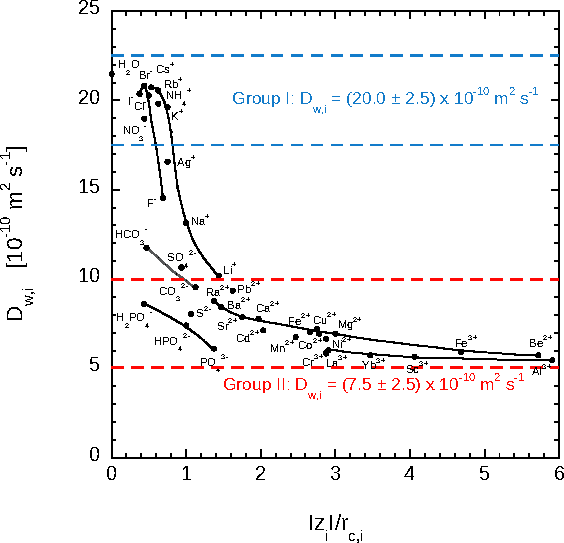
\includegraphics[width=0.6\linewidth]{graphics/free_water_diffusion.pdf}
    \caption{Molecular diffusion in free water, taken from \cite{VanLoon2014_NTB1203}.}
    \label{fig:d_free_water}
\end{figure}

\paragraph{Advection and dispersion in the long-term saturated state.}
Following first-order stochastic theory for macroscopic (field-scale) dispersion (\cite{Zech_Evidence_2023}),
we express the longitudinal macrodispersivity as
\begin{equation}
    \label{eq:dispersivity}
    \alpha_L = \sigma_{\ln K}^2\, I_h,
\end{equation}
where $\sigma_{\ln K}^2=\Var(\ln K)$ is the variance of the log-conductivity field and $I_h$ is the
longitudinal integral scale (defined as the integral of the normalized correlation function along
the mean-flow direction). For the commonly used exponential correlation model, the integral scale
equals the correlation length parameter, and for other standard correlation models, it is of the same
order.

The variance is dimensionless, in particular it is invariant to
the choice of reference conductivity $K_0$:
\[
 \sigma_{\ln K}^2=\Var(\ln K)=\Var\!\bigl(\ln(K/K_0)\bigr),
\]
since $\Var(\ln K_0)=0$ for a constant $K_0$.

The integral scale is expected to be in the range $I_h \approx 0.1$--$1~\mathrm{m}$, associated with
hydration-related inhomogeneities. Using the $\rho_d  \propto \log_{10} K$ relation linear fit, we get:
\[
\sigma_{\log_{10}K} = 6 \sigma_{\rho_d} + 0.08 = 0.26
\]
corresponding to  $\sigma^2_{\ln K}\approx 0.36$.
Then we conclude:
\[
\alpha_L = \sigma_{\ln K}^2 I_h \approx 0.026\text{--}0.26~[m].
\]





\section{Chapter summary}
\label{sec_conclusion}


The distribution of dry density of bentonite pellets in the loading corridors is determined by a combination of the properties of the material, the design parameters of the filling and subsequent hydration. The initial unevenness is significantly reduced over time due to the expansive nature of bentonite and its ability to fill pores, which ensures high efficiency of the insulation and barrier properties of the filling layer and thus the long-term safety of the deep repository.


According to the available information, the backfill in the emplacement drift (Fig.~\ref{fig:image6}) is expected to be placed as pellets, with a macroscopic dry density of $\rho_d = 1400~\mathrm{kg/m^3}$.
The exact method of pellet transportation has not yet been determined. Installation will either be carried out using pneumatic conveying (blowing) or mechanical conveying (belt conveyor, screw conveyor). Achieving the required average dry density of pellets, 
$\rho_d = 1400 \ \mathrm{kg/m^3}$,
can only be assumed when placing an unsorted fraction of \(0\text{–}50 \ \mathrm{mm}\) 
(see Tab.~\ref{tab:compaction}).

For the given fraction \(0\text{–}50 \ \mathrm{mm}\), no measurements of the hydromechanical (HM) parameters of the pellets have been performed under laboratory conditions or under real in situ conditions.

For fully saturated pellets, the HM parameters can be estimated from other measured fractions, e.g., \(0\text{–}8 \ \mathrm{mm}\) (Figs.~\ref{fig:image_hyd_vod} and \ref{fig:image14}), or from the HM parameters of compacted bentonite blocks at the same dry density (Fig.~\ref{fig:image15}).

From these measurements, the hydraulic conductivity and swelling pressure for fully saturated pellets at an average dry density of 
$\rho_d = 1400 \ \mathrm{kg/m^3}$
can be roughly estimated as:
$k = (3.5\text{–}5) \times 10^{-12} \ \mathrm{m/s}, \quad p_s = 1.5\text{–}2.5 \ \mathrm{MPa}$.
For a more accurate determination of swelling pressure and hydraulic conductivity values, several measurements should be carried out at \(\rho_d = 1400 \ \mathrm{kg/m^3}\).


\paragraph{Heterogenities and possible preferential pathways:}
Density gradients during emplacement may form transient preferential pathways.  
Upon saturation, swelling of pellets closes the upper voids and homogenises the 
backfill structure. The resulting radial stress $p_r$ contributes to closure of \Gls{EDZ} 
microfractures and reduction of its hydraulic conductivity. Long-term preferential 
path formation is therefore unlikely once full saturation is reached.

From the perspective of possible preferential flow paths (zones with higher hydraulic conductivity) in the backfill, it is necessary to know the input parameters for HM modelling of unsaturated flow in pellets of the required fraction (\(0\text{–}50 \ \mathrm{mm}\)). For pellets made from Czech unsaturated bentonite \acrshort{BCV}, no measurements have been carried out in this regard. An overview of comprehensively measured input HM parameters and methods for measuring partially saturated pellets can be found in the literature (\cite{Hoffmann2007hydro}), concerning FEBEX pellets.

When backfilling a drift with a height of \(6.7 \ \mathrm{m}\) (Fig.~\ref{fig:image6}) using pellets, self-compaction is expected to cause a decrease in dry density towards the top, resulting in the formation of a void space in the upper part. Moreover, the weight of bentonite cause a compation of pellets in lower domains by gravity. Therefore, it would be appropriate to prepare a \(1{:}1\) scale experiment for pellet transportation into a model drift and measure the distribution of pellet density and any possible void formation at   the top.


\paragraph{Pellet vs. Compact Block comparison:}
In practical backfill systems, pellet fills are usually used in the gaps between compacted blocks. Compared to monolithic blocks, a pellet layer has lower swelling pressure and water uptake per unit volume when initially unsaturated. For instance, \cite{villar2021febex} note that a pellet mixture at a given dry density develops a “double-peak” swelling response: an initial modest swelling as pellets expand, followed by a slower increase as the mix densifies, whereas a compacted block yields a single larger peak pressure. However, once fully saturated, a pellet fill can reach similar final swelling stress as the blocks. In terms of water retention, the key difference is exactly that: a pure block (or fine powder) holds more capillary water at moderate suction than a loose pellet mix \cite{villar2021febex, mesa2020microstructural}. Therefore, during early saturation a pellet backfill may carry a lower degree of saturation at a given hydration stage. Nonetheless, SKB/Posiva modeling assumes that any initial moisture heterogeneity (pellets vs blocks) will eventually homogenize as water migrates; the long-term barrier performance (tightness) is then governed by the overall final density and saturation, which for an optimally swelled pellet/block fill remains high.






% ---------------------------------
\section{Appendix \ref*{ch:bentonite}A: EB experiment – dry density gradient}
\label{sec_append1}

As part of monitoring the filling, for example in the \textit{EB experiment} (Fig.~\ref{fig:image18}), a significant gradient of the initial dry density of pellets was observed when filling the access tunnel with a screw conveyor. It was found that larger pellets filled the lower parts faster and prevented smaller particles from effectively filling the gaps. As a result, the difference in dry density was measured from approximately $1.25 \munit{Mg/m^3}$ in the lower layers to $1.45 \munit{Mg/m^3}$ in the upper part. This effect is important for the design of the optimal granulometry of the pellets and the filling methodology.
\begin{figure}[!htbp]
  \centering
  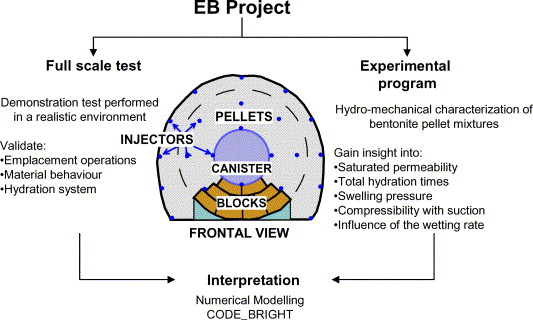
\includegraphics[width=0.7\textwidth]{graphics/img_ugn/image18.jpeg}
\caption{The scheme of EB experiment.}
  \label{fig:image18}
\end{figure}

\begin{figure}[htbp]
    \centering
    \begin{subfigure}{0.45\textwidth}
        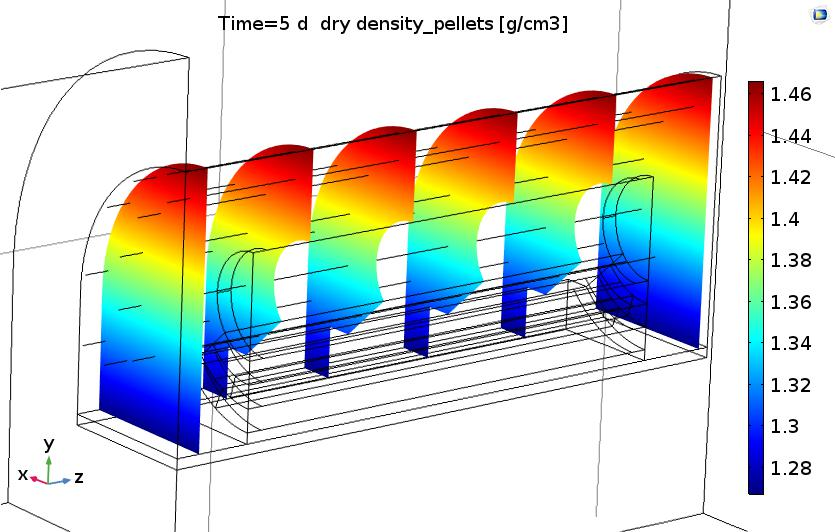
\includegraphics[width=\linewidth]{graphics/img_ugn/image19.jpg}
        \caption{Dry density at the beginnig of the EB experiment in the pellet space.}
    \end{subfigure}
    \begin{subfigure}{0.45\textwidth}
        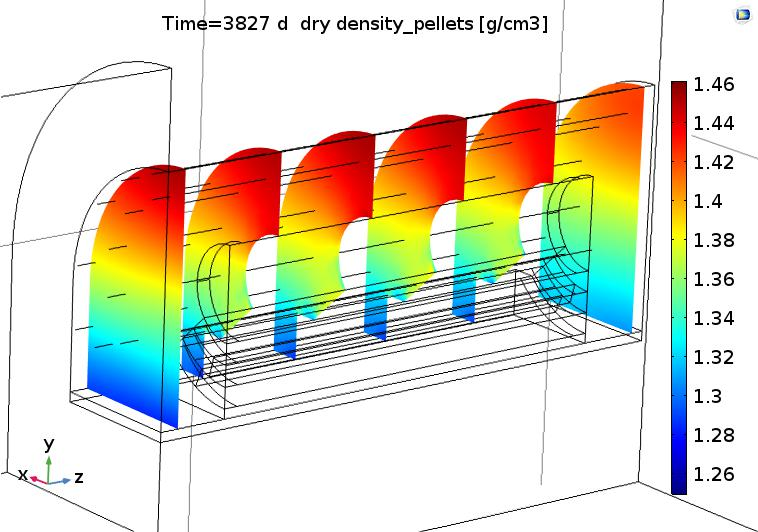
\includegraphics[width=\linewidth]{graphics/img_ugn/image20.jpeg}
        \caption{Dry density at the end of the EB experiment in the pellet space.}
    \end{subfigure}
    
    \vspace{0.5cm}
    
    \begin{subfigure}{0.45\textwidth}
        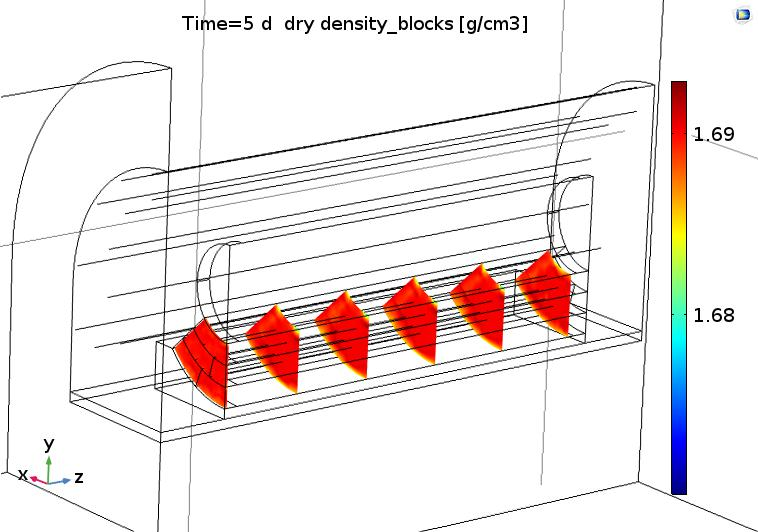
\includegraphics[width=\linewidth]{graphics/img_ugn/image21.jpeg}
        \caption{Dry density at the beginnig of the EB experiment in bentonite blocks.}
    \end{subfigure}
    \begin{subfigure}{0.45\textwidth}
        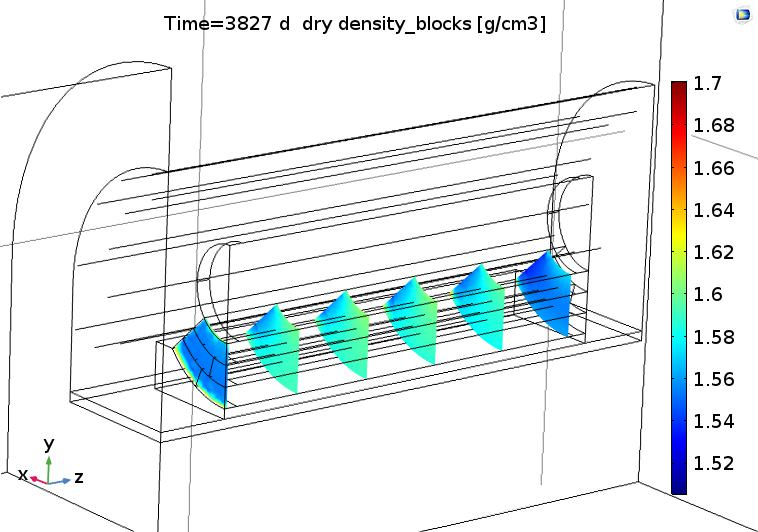
\includegraphics[width=\linewidth]{graphics/img_ugn/image22.jpeg}
        \caption{Dry density at the end of the EB experiment in bentonite blocks.}
    \end{subfigure}
    \caption{Distribution of dry density in EB experiment.}
    \label{fig:2x2EB}
\end{figure}



The pellet space did not change significantly. There was a small compression of the pellets due to the expansion of the bentonite blocks and the associated vertical movement of the steel cylinder (change in the average $\rho_d$ of the pellets at the beginning $1.36 \munit{Mg/m^3}$ at the end of the EB experiment $1.38 \munit{Mg/m^3}$, change in the average $\rho_d$ of the blocks at the beginning $1.69 \munit{Mg/m^3}$ at the end of the EB experiment to $1.58 \munit{Mg/m^3}$). 

Dismantling was started in October 2012 and completed in January 2013. In doing so, many high-quality data were obtained on the final state of the barrier (especially water content, density, and degree of saturation, hydraulic conductivity). Information on the \Gls{EDZ} before and after dismantling is also available. An idea of the information obtained is given in Fig.~\ref{fig:image23}.

\begin{figure}[!htbp]
  \centering
  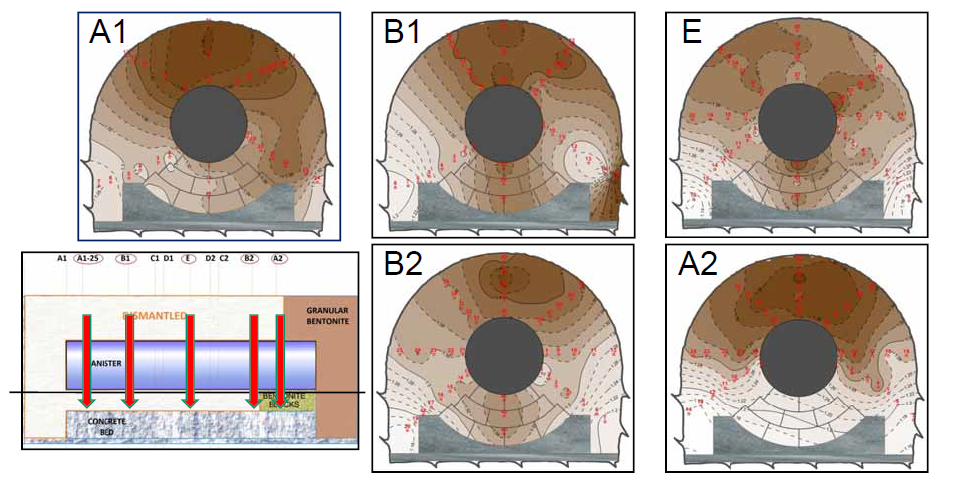
\includegraphics[width=0.8\textwidth]{graphics/img_ugn/image23.png}
\caption{Heterogeneity of dry density in selected sections (\cite{palacios2013eb}).}
  \label{fig:image23}
\end{figure}

% ----------------------------------------------
\section{Appendix \ref*{ch:bentonite}: EBS Task 13 Stage 2}
\label{sec_append2}

In the Stage~2 experiment, bentonite at an initial dry density of approximately 
$\rho_d = 1.65$ – $1.69 \ \mathrm{g/cm^3}$
was saturated with liquid-phase water at a very low flow rate from the bottom surface, opposite to the location of the gap (see Fig.~\ref{fig:image26}).  
The specimen diameter was \(5.0 \ \mathrm{cm}\) and its height was \(2.52\text{–}2.58 \ \mathrm{cm}\).  
The initial height of the gap was approximately \(0.9 \ \mathrm{cm}\).  

The specimen was placed between porous stones, and the top part of the stainless steel cell above the gap was open to the atmosphere. Demineralized water was injected through the bottom via a pressure/volume regulator at a rate of
$Q = 0.07 \ \mathrm{cm^3/h}$,
while the injection pressure was measured (identical for both types of tests). At the start of the tests, the injection pressure was atmospheric. All experiments were carried out at laboratory temperature
$T = 22.5 \pm 1.3 \ ^\circ\mathrm{C}$.
EBS Task 13 Stage 2 gave the results for six dismantled specimens.

\begin{figure}[!htbp]
  \centering
  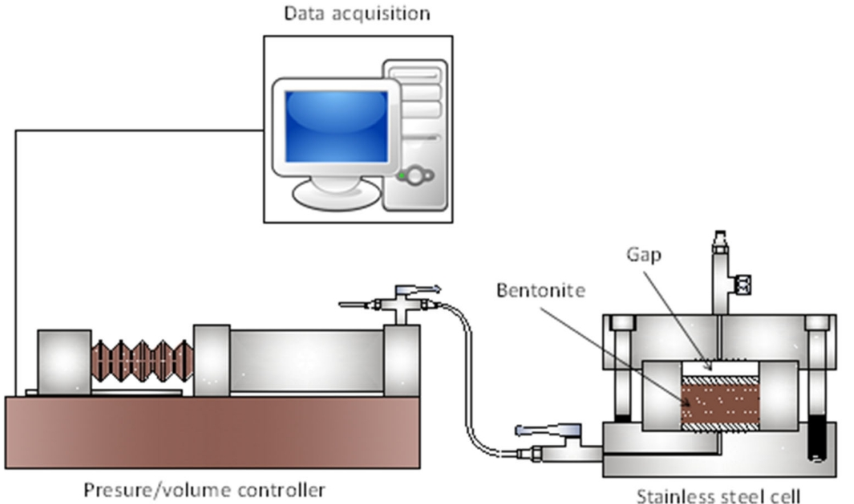
\includegraphics[width=0.6\textwidth]{graphics/img_ugn/image26.png}
\caption{Schematic representation of the Stage 2 test setup.}
  \label{fig:image26}
\end{figure}

At the end of all types of tests (after different time periods), the specimens were measured, weighed, and cut into vertical sections (see Fig.~\ref{fig:three_in_row}). From each section, subsamples were taken to determine water content, dry density, and mass. Typically, three zones (Fig.~\ref{fig:three_in_row}, right) of a given size were defined, since a minimum section volume was required to obtain sufficiently continuous subsamples for accurate dry density determination.

\begin{figure}[!htbp]
\centering
\begin{subfigure}[t]{0.32\textwidth}
    \centering
    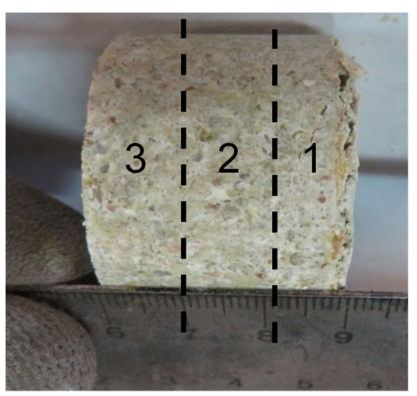
\includegraphics[width=\textwidth]{graphics/img_ugn/image27.png}
\end{subfigure}
\hfill
\begin{subfigure}[t]{0.32\textwidth}
    \centering
    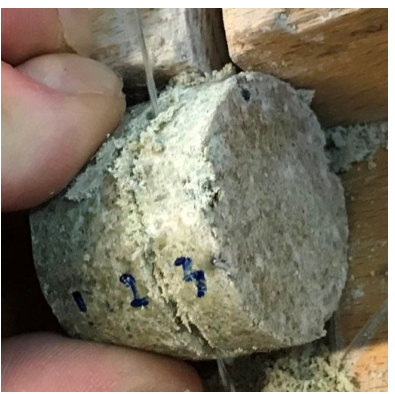
\includegraphics[width=\textwidth]{graphics/img_ugn/image28.png}
\end{subfigure}
\hfill
\begin{subfigure}[t]{0.32\textwidth}
    \centering
    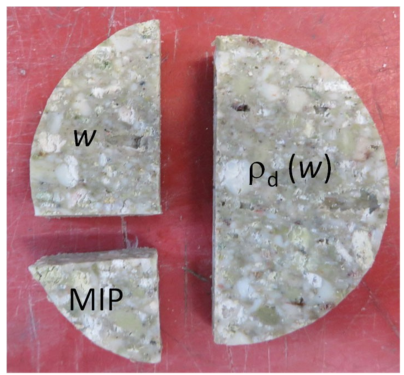
\includegraphics[width=\textwidth]{graphics/img_ugn/image29.png}
\end{subfigure}
\caption{Final sub-sampling after extraction of samples from Stage 2 test cells. Sub-sampling of the section for post-mortem determination (right).}
\label{fig:three_in_row}
\end{figure}

The dry density, \(\rho_d\), is defined as the ratio between the mass of the dry specimen and the volume it occupied prior to drying:
$\rho_d = \frac{m_{\mathrm{dry}}}{V_{\mathrm{initial}}}$.

The volume of the specimens after removal from the cell was determined by measuring their dimensions, while the volume of subsamples from each section was obtained by immersion into a container filled with mercury and weighing the displaced mercury, assuming a mercury density of
$\rho_{\mathrm{Hg}} = 13.6 \ \mathrm{g/cm^3}$.

The water content was determined for the subsamples used for \(\rho_d\) determination as well as for an additional subsample from each section. The gravimetric water content \(w\) is defined as the ratio between the mass of water and the mass of the dry specimen, expressed as a percentage:
\[
w \ [\%] = \frac{m_{\mathrm{water}}}{m_{\mathrm{dry}}} \times 100.
\]
The mass of water, \(m_{\mathrm{water}}\), was obtained as the difference between the total mass of the specimen, \(m_{\mathrm{total}}\), and its dry mass after oven-drying at \(110 \ ^\circ\mathrm{C}\) for 48 hours:
$m_{\mathrm{water}} = m_{\mathrm{total}} - m_{\mathrm{dry}}$.

A total of six tests were performed on specimens with the same initial properties, which were dismantled after different hydration periods (Table~\ref{tab:stage2}). All specimens were weighed both at installation and upon completion of the tests.


\begin{table}[!htbp]
\centering
\caption{Initial and final characteristics of Stage 2 tests with hydration from the bottom.}
\label{tab:stage2}
\resizebox{\textwidth}{!}{%
\begin{tabular}{lccccccccccc}
\hline
\textbf{Test} & \textbf{Duration} & \textbf{Initial} & \textbf{Initial} & \textbf{Initial} & \textbf{Initial} & \textbf{Initial} & \textbf{Final} & \textbf{Final} & \textbf{Final} & \textbf{Final} & \textbf{Final} \\
 & (days) & $w$ (\%) & $\rho_d$ (g/cm$^3$) & $S_r$ (\%) & sample $h$ (cm) & gap $h$ (cm) & $w$ (\%) & $\rho_d$ (g/cm$^3$) & $S_r$ (\%) & sample $h$ (cm) & gap $h$ (cm) \\
\hline
GL1  & 63 & 13.3 & 1.65 & 57 & 2.58 & 0.83 & 45.2 & 1.25 & 103 & 3.41 & 0.00 \\
GL2  & 14 & 13.3 & 1.67 & 59 & 2.54 & 0.87 & 32.2 & 1.32 & 83  & 3.21 & 0.20 \\
GL3  & 28 & 13.8 & 1.67 & 60 & 2.53 & 0.90 & 44.9 & 1.23 & 102 & 3.43 & 0.00 \\
GL4  &  7 & 14.3 & 1.67 & 62 & 2.52 & 0.89 & 24.1 & 1.50 & 81  & 2.81 & 0.60 \\
GL5  &  4 & 14.4 & 1.66 & 62 & 2.55 & 0.85 & 18.9 & 1.58 & 72  & 2.69 & 0.70 \\
GL12 & 10 & 13.1 & 1.69 & 59 & 2.52 & 0.90 & 26.3 & 1.43 & 80  & 2.98 & 0.44 \\
\hline
\end{tabular}%
}
\end{table}

During the experiments, it was possible to accurately determine the amount of water that entered the samples during the hydration process.  
Tests GL2, GL4, GL5, and GL12 did not reach full saturation due to the short test duration, whereas tests GL1 and GL3 were fully saturated at the end of the experiments.  
In all cases, the upper air outlet remained open to the atmosphere throughout the entire test duration.

The water content $w$ and dry density $\rho_d$ at different levels of the samples, measured at the end of the tests, are shown in Figure~\ref{fig:image31}.  
The total water content increased over time, but was always higher near the hydration surface.  
Similarly, the dry density $\rho_d$ of the bentonite decreased as the gap was filled, and it was always lower near the hydration surface.  
Lower dry density implies higher permeability $k$ (i.e., higher hydraulic conductivity).  

Although the gradients decreased over time, they did not disappear, even when the sample became fully saturated;  
the water content $w$ remained higher, and the bentonite dry density $\rho_d$ remained lower, in the vicinity of the hydration surface for tests GL1 and GL3.


\begin{figure}[!htbp]
  \centering
  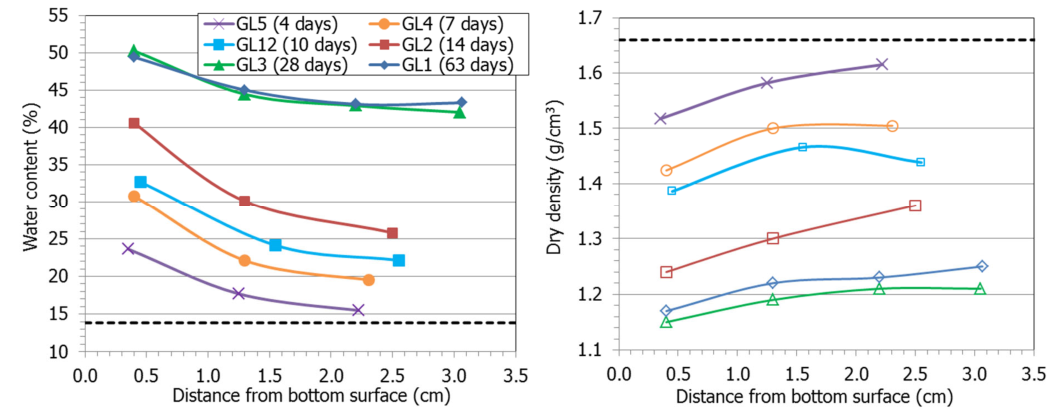
\includegraphics[width=0.8\textwidth]{graphics/img_ugn/image31.png}
\caption{Schematic representation of the Stage 2 test setup.}
  \label{fig:image31}
\end{figure}





